% !TeX root = ../main.tex
\chapter{检测平台设计}\label{ch:rig}

本章以上一章提出的改进方案为基础,讨论大气环境下的静电卡盘静电力检测平台的设计。由于检测平台是一个复杂的机、电、气相结合的系统,本章首先分析检测平台所需具有的功能与组成部分,然后提出其总体设计方案,最后分组件讨论检测平台各部分的具体设计。



\section{总体设计方案}\label{sec:rig-overall}

根据已有背吹平衡方案,以及\ref{principle-soln}节中提出的改进措施(主要是微力探头),确定检测平台必须具有的功能如下:对静电卡盘背吹通道气压的控制与检测、对微力探头的定位与受力检测、检测过程的自动控制、数据采集与储存等。据此,可将整个平台划分为图~\ref{fig:rig-overall-sch}所示的几大组成部分:

\begin{figure}[tbh]
\centering
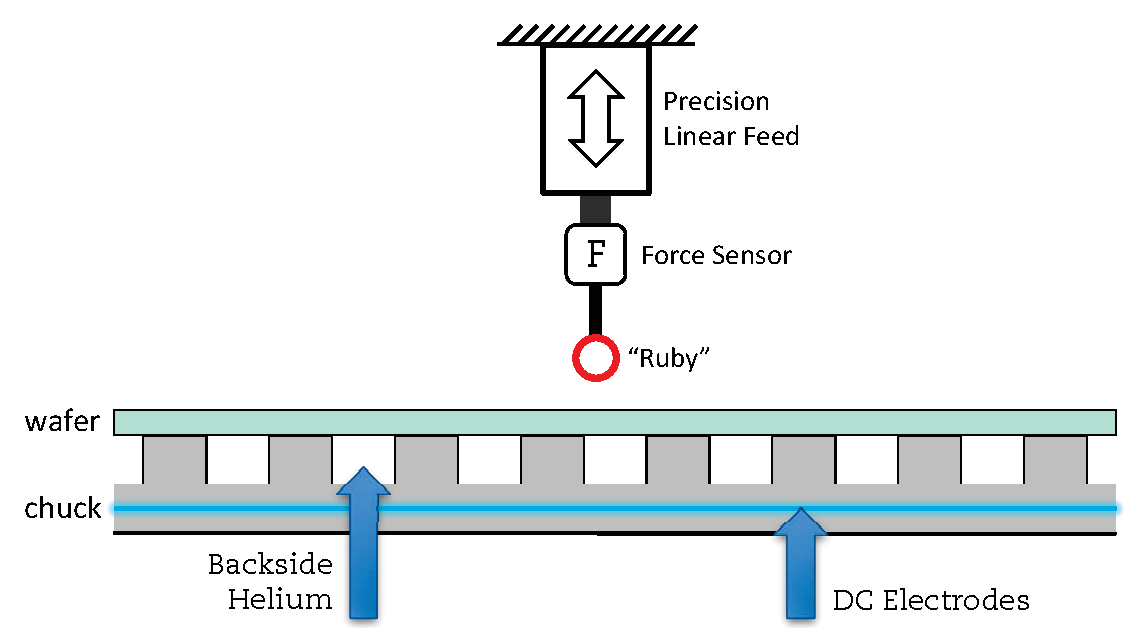
\includegraphics[width=1\linewidth]{rig/overall__sch}
\caption{测量平台总体设计方案示意}
\label{fig:rig-overall-sch}
\end{figure}

\begin{enumerate}
  \item \textbf{待测静电卡盘及其配套静电电源} :
    待测静电卡盘为北方微电子公司提供的一台\SI{300}{mm}双极型静电卡盘,如图~\ref{fig:rig-overall-chuck},采用埋在氮化铝陶瓷层中的交叉环形金属电极。其陶瓷层表面均布圆形小凸台,边缘处有宽约\SI{2}{\milli\meter}的环形凸起,共同形成背吹通道。配套的直流静电电源可通过标准接头与静电卡盘两电极相连,提供高达\SI{3000}{\volt}的静电电压。
  \item \textbf{微力探头组件} :
    图~\ref{fig:rig-overall-sch}中位于卡盘上方的部分即为微力探头组件,其主体为\ref{principle-soln-ruby}节所述的微力探头。详细设计在\ref{sec:rig-probe}节讨论。
  \item \textbf{背吹控制系统} :
    向静电卡盘背吹通道提供稳定、可控的气压,并检测背吹通道入口处气压值。详细设计在\ref{sec:rig-pressure}节讨论。
  \item \textbf{机械结构} :
    为所有其他组件(包括配管配线等)提供定位、支撑作用。详细设计在\ref{sec:rig-model}节讨论。
  \item \textbf{自动控制与数据采集系统} :
    包括微力探头组件与背吹控制系统中的接口电路、总控单元、以及PC三大部分,主要功能为自动控制整个检测过程,采集各传感器数据,并将其传输到PC中储存。详细设计在\ref{sec:rig-ctrl}节讨论。
\end{enumerate}

\begin{figure}[p]
\centering
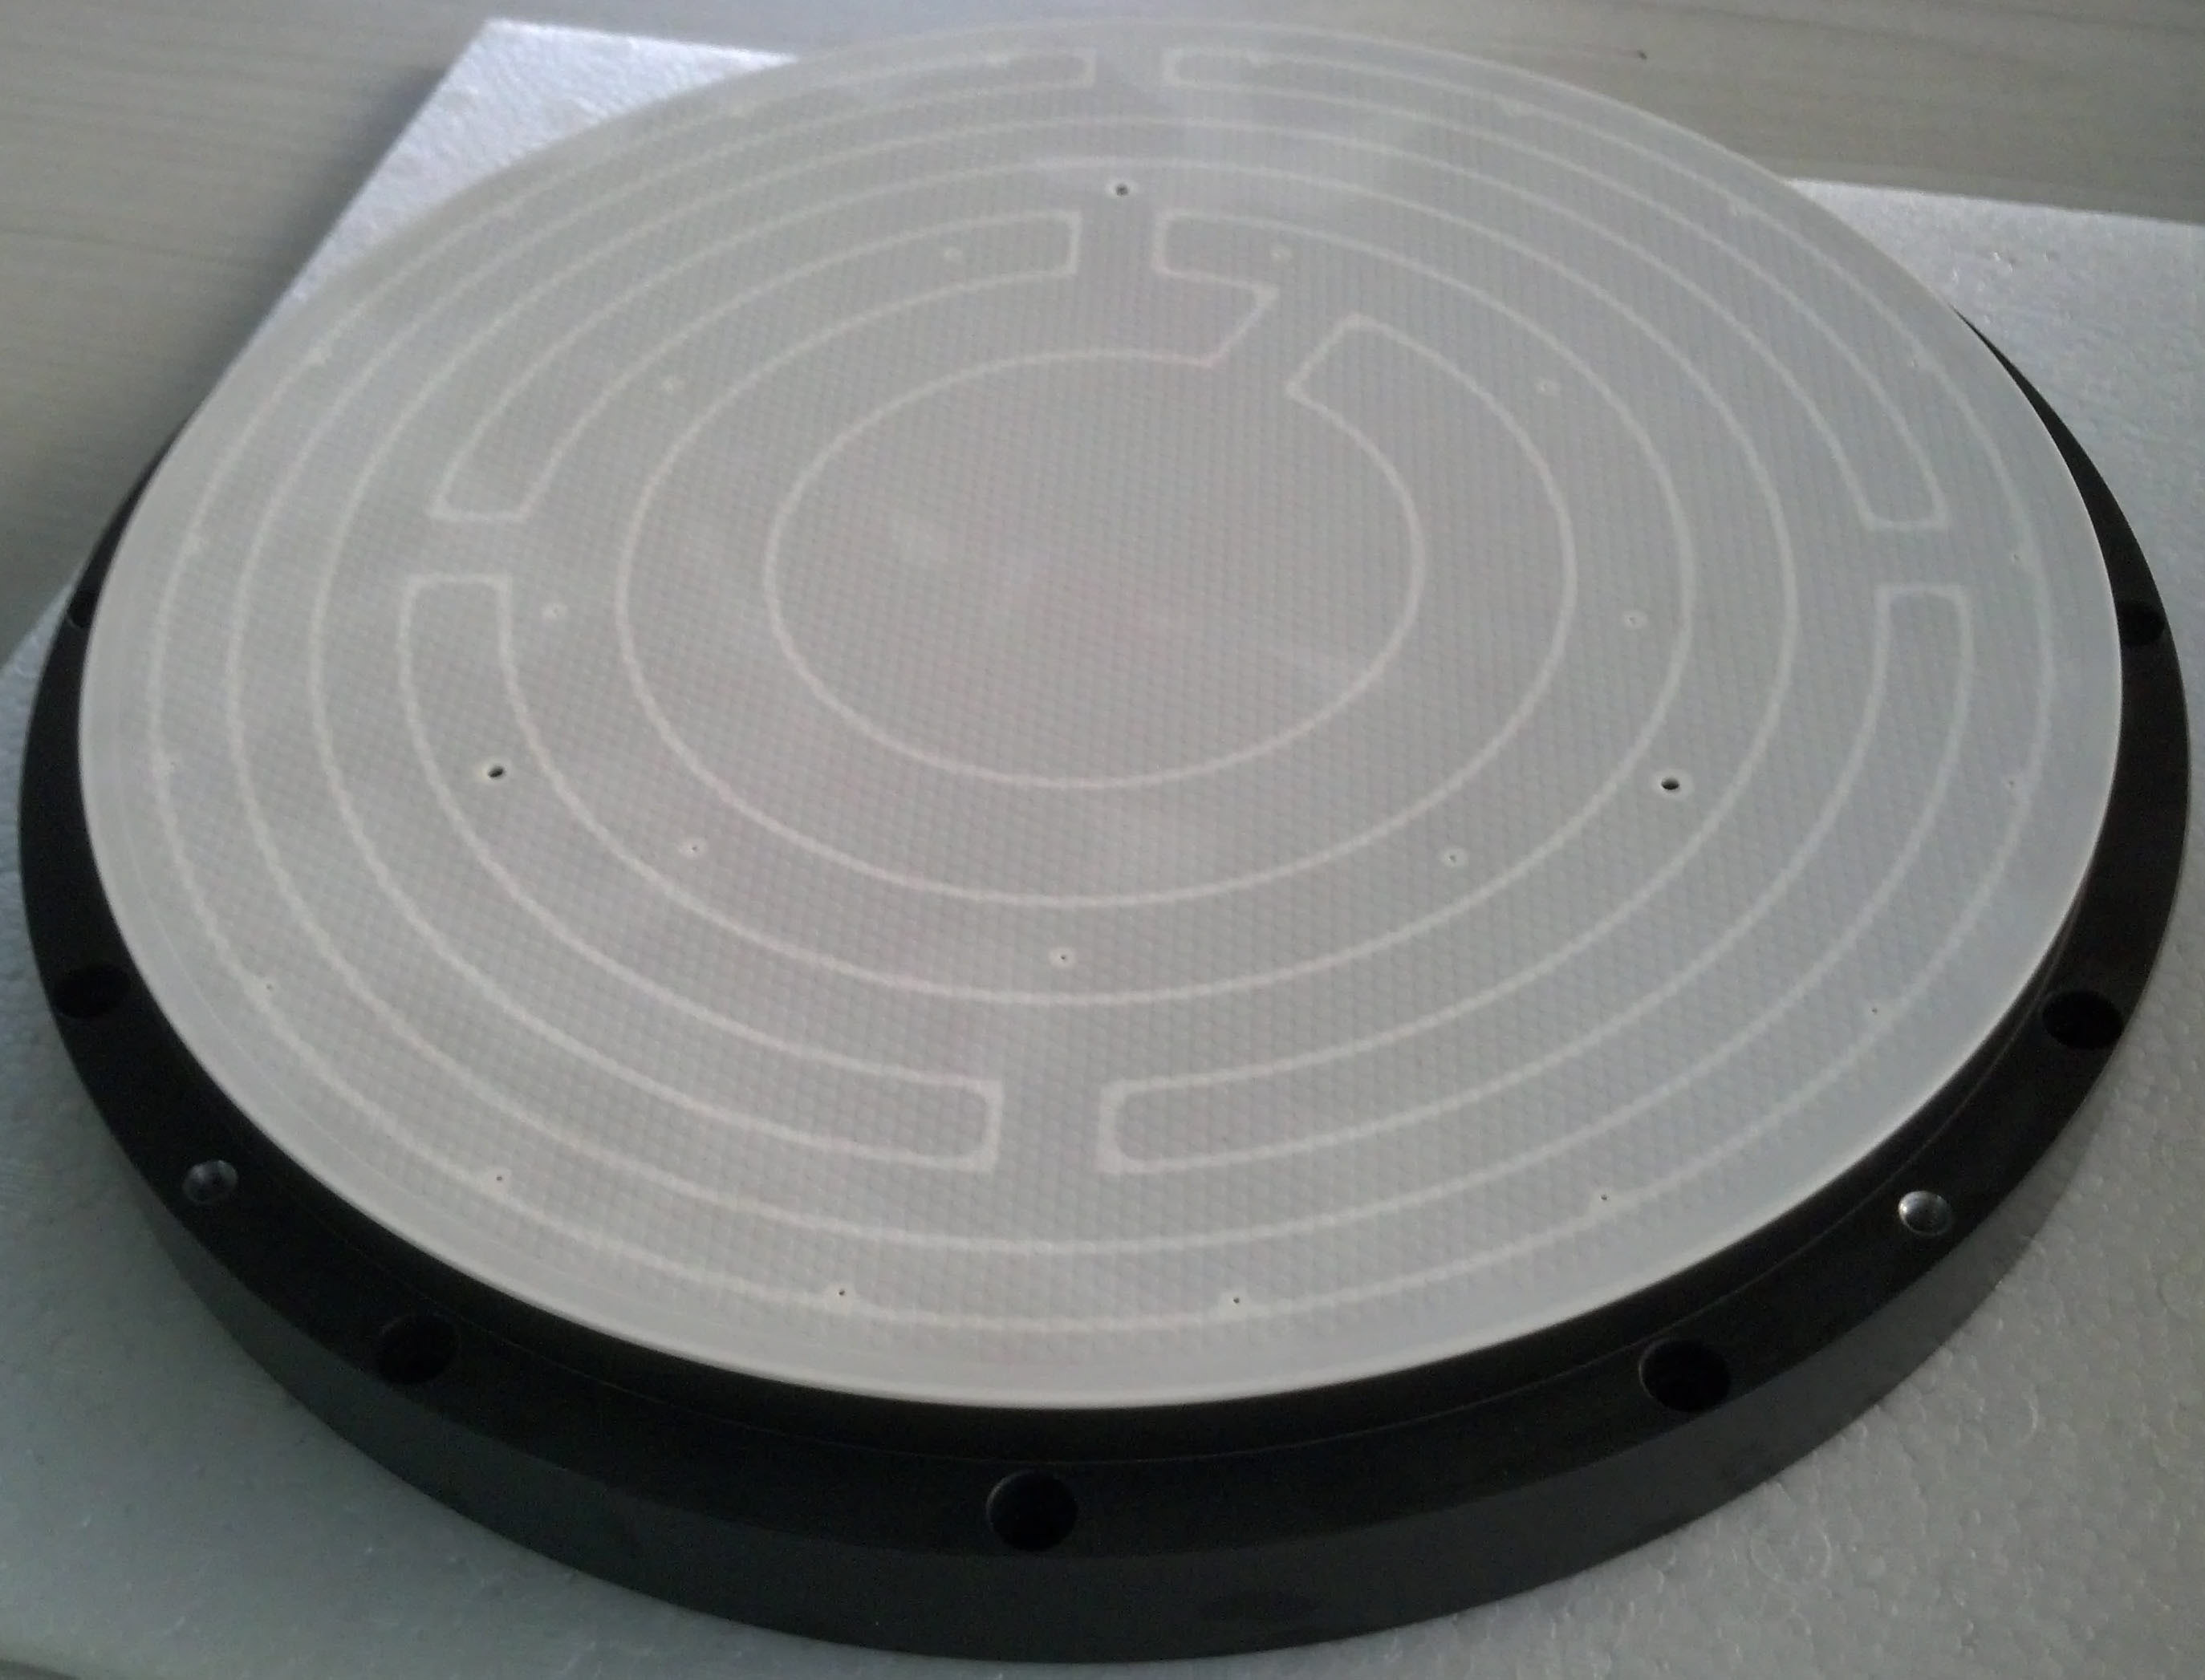
\includegraphics[height=0.40\textheight]{rig/overall__chuck__front.jpg} \\
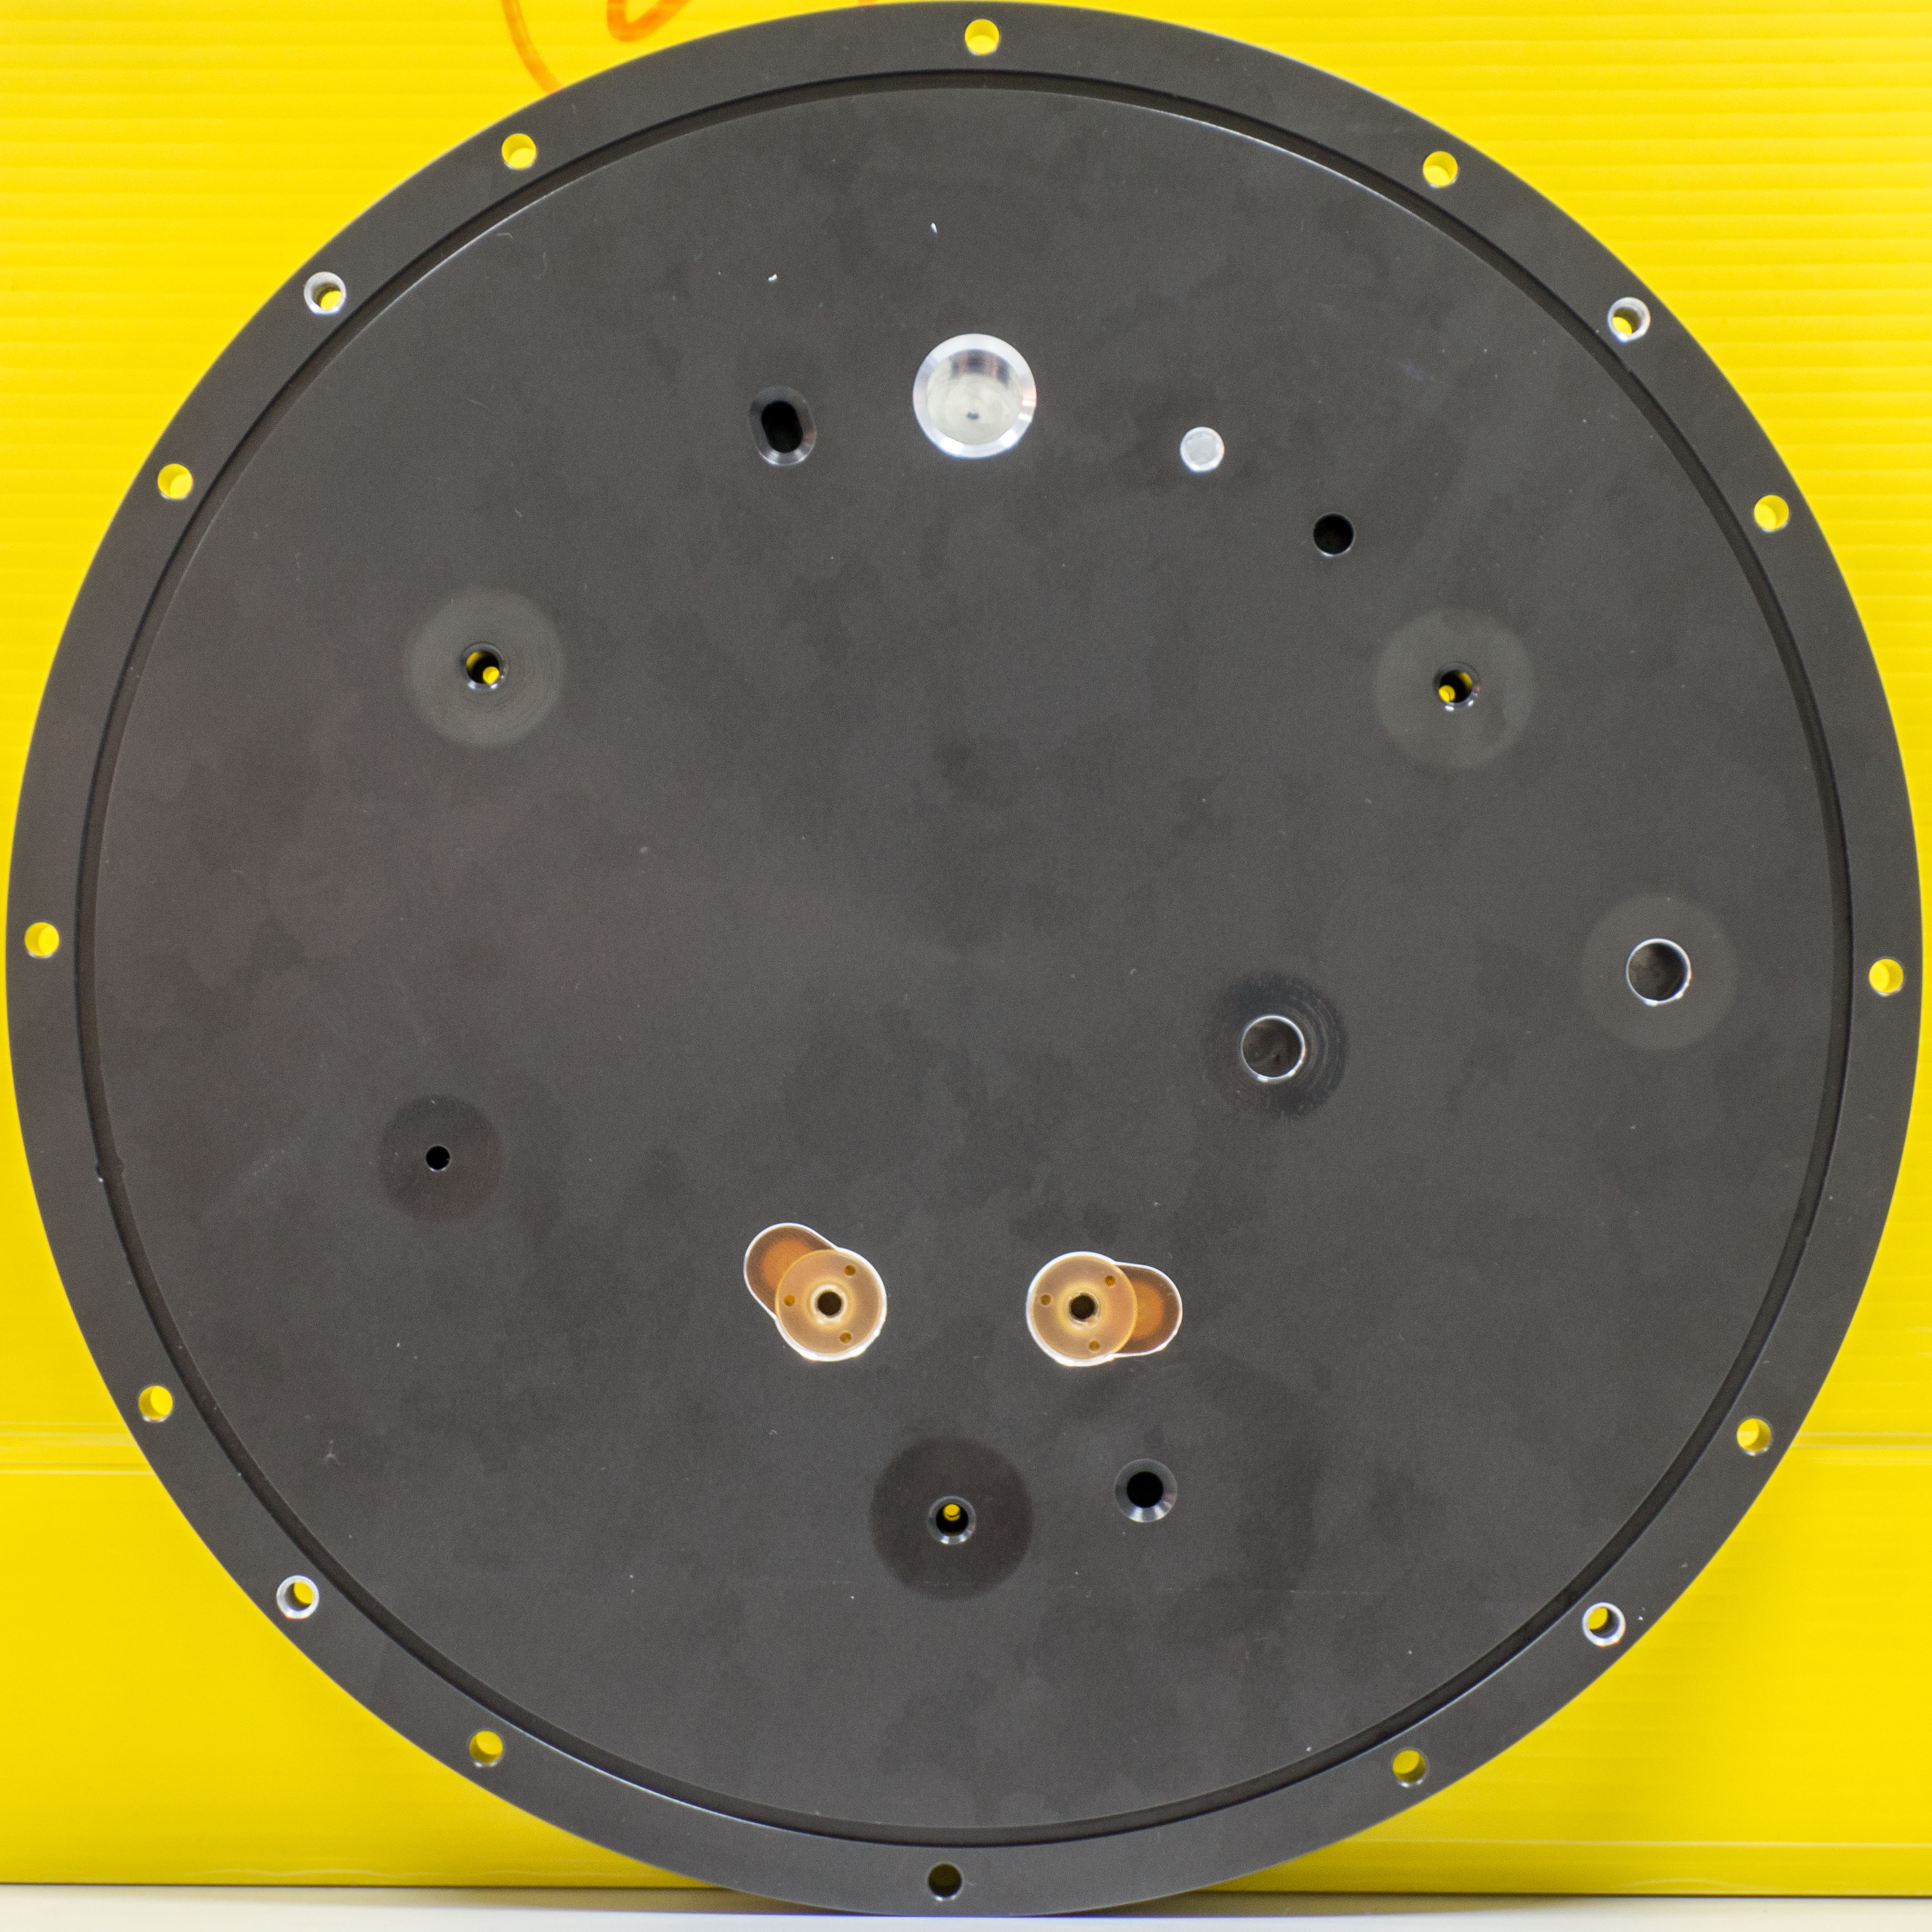
\includegraphics[height=0.50\textheight]{rig/overall__chuck__back.jpg}
\caption{待测静电卡盘}
\label{fig:rig-overall-chuck}
\end{figure}



\clearpage



\section{微力探头组件设计}\label{sec:rig-probe}

\ref{principle-soln-ruby}节中提出了由微力传感器和红宝石探头组成的微力探头。该探头需在晶圆吸附后与晶圆接触,并保证接触力$N_{\mathrm{probe}} \ll F_{\mathrm{elec}}$。这可通过增设精密直线进给机构实现。具体方法如下:将微力探头组件连接到进给机构的移动端,进给机构的固定端连接在检测平台框架上,如图~\ref{fig:rig-overall-sch}。晶圆吸附后,驱动进给机构向靠近晶圆方向缓缓移动,同时通过微力传感器监测$N_{\mathrm{probe}}$;当$N_{\mathrm{probe}}$测量值明显增加,超过一定阈值\footnotemark{}时,立即停止进给机构运动,则此时$N_{\mathrm{probe}}$大小由阈值、传感器刚度、进给速度、进给机构特性共同决定,只要参数选取合适,即可保证$N_{\mathrm{probe}} \ll F_{\mathrm{elec}}$。

\footnotetext{该阈值可人为根据传感器特性确定,也可通过数字信号处理方式动态获得,甚至可采用阈值判定以外的其他方式,在此不再赘述。}

微力探头组件中,红宝石探头可直接从标准三坐标测量机探头组中选取,而微力传感器与进给机构需外购。本节主要讨论两外购件的选型。


\subsection{微力传感器选型}\label{sec:rig-probe-sensor}

微力传感器是探头组件中的核心元件,由上文讨论知,其关键参数与系统性能直接相关,且影响进给机构的选型,因此需首先确定其选型。本节通过对检测过程的分析,先估测关键参数的范围,以此为标准筛选出备选产品,最后对比评估选择合适的微力传感器。

量程是微力传感器最主要的参数,所有相对性能指标均以满量程为基准,如精度、分辨力、敏感度等。合理的量程选择应完全覆盖传感器在整个检测过程中受力的范围,但又不超过该范围过多,以保证测量精度,减小噪声干扰。由于检测过程中需一直保证$N_{\mathrm{probe}} \ll F_{\mathrm{elec}}$,而保守估计静电力$F_{\mathrm{elec}}$在$\SIrange{5}{200}{\newton}$范围内,若设定1\%作为“远小于”的上界(即$N_{\mathrm{probe}} \leq 0.01 \cdot F_{\mathrm{elec}}$),则$N_{\mathrm{probe}} \leq \SI{0.05}{\newton}$,由此确定传感器量程合理取值范围为$\SIrange{0.05}{0.5}{\newton}$。确定量程后,还需确定与其直接相关的安全过载范围。考虑到在安装、调试过程中,以及硅晶圆突然完全脱附时,探头均可能瞬间受到较大的力的作用,若微力传感器具有较大安全过载范围,则可避免意外受损。保守估计传感器需至少能承受\SI{0.5}{\newton}量级的瞬间轴向压缩力而性能不受影响。

为了准确检测脱附,需要传感器能分辨较小的受力增量,即具有高分辨力。一般分辨力标称值为满量程的百分比(\% FS),在比较量程不同的传感器时,需先将其转换为绝对数值。当传感器未标称分辨力时,可参考其重复精度数据。由于传感器分辨力越高,成本也越高,根据静电力范围粗估\SI{0.25}{\milli\newton}作为分辨力的参考数值。%TODO:more reasoning

另外,由\ref{principle-soln-ruby}节中关于晶圆挠度的讨论,在其他条件不变的情况下,传感器刚度$k$越高,晶圆挠度范围越小,但同时越难控制探头与晶圆的初始接触力(见上文中保证接触力方法,以及\ref{sec:rig-probe-feeding}节\eqref{eq:rig-probe-feeding-vel}式)。因此,挠度取值及其对检测的影响需作为选型时的重要参考。

表~\ref{tab:rig-probe-sensor}为初步筛选后的选型表。若考虑量程、精度、分辨力,1050V1较差;若考虑刚度,LSB200较差;若考虑过载性能,FT-S10000较差。综合考虑,LSB200在量程、过载范围、重复精度等方面与预期符合最好,因此选择该产品。

% generated using http://www.tablesgenerator.com/latex_tables
\begin{table}[htbp]
\begin{minipage}{1\linewidth}
\centering
\caption{微力传感器选型表}
\label{tab:rig-probe-sensor}
\begin{tabular}{@{}lllccc@{}}
\toprule[1.5pt]
生产商 &  &  & Futek & Dytran & FemtoTech \\
型号 &  &  & LSB200 & 1050V1 & FT-S10000 \\
\midrule[1pt]
原理 &  &  & 应变式 & 压电式 & MEMS \\
输出信号 & 类型 &  & 电阻电桥 & 电压 & 电压 \\
 & 单位 &  & \si{\milli\volt\per\volt} & V & V \\
灵敏度 & 满量程 & 输出 & 0.5 & 5 & 2 \\
 & 单位受力 & 输出/\si{\newton} & 5.0E+00 & 1.1E-01 & 2.0E+02 \\
分辨力 &  & \si{\micro\newton} & --\footnote{未标称,按重复精度估计} & 600 & 0.5 \\
刚度 &  & \si{\newton\per\micro\meter} & 0.001 & 1996.45 & --\footnote{未标称,但考虑到其原理,估计其挠度为\SI{1}{\micro\meter}量级} \\
\midrule[1pt]
满量程 & 拉(+) & \si{\newton} & 0.1 & 44.48 & 0.01 \\
 & 压(-) & \si{\newton} & 0.1 & 44.48 & 0.01 \\
最大载荷 & 拉(+) & \si{\newton} & 1 & 889.64 & 0.03 \\
 & 压(-) & \si{\newton} & 1 & 889.64 & 0.03 \\
\midrule[1pt]
线性度 &  & \% FS & 0.1 & 1 & \multirow{2}{*}{--}\footnote{未标称,考虑到其分辨力,可按0.1\%估计,下同} \\
 &  & \si{\newton} & 2.00E-04 & 8.90E-01 &  \\
滞回 &  & \% FS & 0.1 & \multirow{2}{*}{--} & \multirow{2}{*}{--} \\
 &  & \si{\newton} & 2.00E-04 &  &  \\
重复精度 &  & \% FS & 0.05 & \multirow{2}{*}{--} & \multirow{2}{*}{--} \\
 &  & \si{\newton} & 1.00E-04 &  &  \\
\bottomrule[1.5pt]
\end{tabular}
\end{minipage}
\end{table}


\clearpage


\subsection{精密直线进给机构选型}\label{sec:rig-probe-feeding}

精密直线进给机构按其驱动方式可分为手动、电动两类,按其移动部分的构造可分为推杆、滑移台两类。为了实现检测过程的自动化,减小人操作产生的随机误差,选用电动进给机构(手动进给机构可作为备用方案)。本节采取与上一节相同思路讨论电动进给机构的选型。

由上文讨论,该进给机构在检测过程中的主要作用为控制探头与晶圆接触,且保证接触力大小在规定范围内。这要求进给机构能在低速下平稳运动,无爬行现象,且速度波动尽量小。下面通过分析接触过程,估计对进给机构运动速度的要求。
%TODO:add schematic?
在进给机构、微力探头与晶圆组成的系统中,由于只有微力传感器的刚度远低于其他所有组件,可将晶圆等效为一固定平面,微力传感器等效为一与传感器同刚度的理想弹簧,进给机构等效为匀速向下运动的弹簧一端。由于进给机构负载非常小,可以认为弹簧上端可瞬间加减速。设$k$为弹簧刚度,$F$为弹簧受力(即$N_{\mathrm{probe}}$),$v$为弹簧上端运动速度,从$F = F_{\mathrm{thres}}$(即传感器受力超过阈值)开始到弹簧上端停止运动的总延迟为$\Delta t$,则根据胡克定律,停止时有:
\begin{equation}
\label{eq:rig-probe-feeding-force}
F = F_{\mathrm{thres}} + k v \Delta t \leq F_{\max}
\end{equation}
解$v$得:
\begin{equation}
\label{eq:rig-probe-feeding-vel}
v \leq \frac{ F_{\max} - F_{\mathrm{thres}} }
            { k \Delta t }
\end{equation}
LSB200刚度$k = \SI{0.001}{\newton\per\micro\meter}$,取$F_{\max}$为LSB200重复精度的10倍,即\SI{1}{\milli\newton},粗估$t_{\mathrm{delay}} = \SI{0.01}{\second}$。将以上数据代入\eqref{eq:rig-probe-feeding-vel}式,得:
\[
v \leq \SI{100}{\micro\meter\per\second}
\]
因此,进给机构需能至少在\SI{100}{\micro\meter\per\second}的速度下平稳运行。

微型精密电动进给机构行程较短,为方便检测平台装配与使用,可设计粗精二级调节:先使用一级粗动台(手动或电动均可)将整个微力探头组件定位在距晶圆不超过精密进给机构行程的位置上,再驱动精密进给机构控制探头与晶圆接触。为了减小对粗调环节要求,需要精密进给机构行程至少为\SI{5}{\milli\meter}。

由于候选型号较多,完整的选型表参见附录B。
%TODO:xref appendix (feeding mashup)
综合考虑性能、价格、订货周期等因素,选择LAC10A-T4精密电动推杆(图~\ref{fig:rig-probe-feeding-LAC10A}),其原理为步进电机驱动滚珠丝杠,有效行程\SI{10}{\milli\meter},重复定位精度$\pm\SI{1.5}{\micro\meter}$。另外,选择JYPY-02213精密手动滑移台(图\ref{fig:rig-probe-feeding-JYPY})作为备用方案,其行程\SI{13}{\milli\meter},测微螺旋最小刻度\SI{10}{\micro\meter}。

\begin{figure}[tbh]
\centering
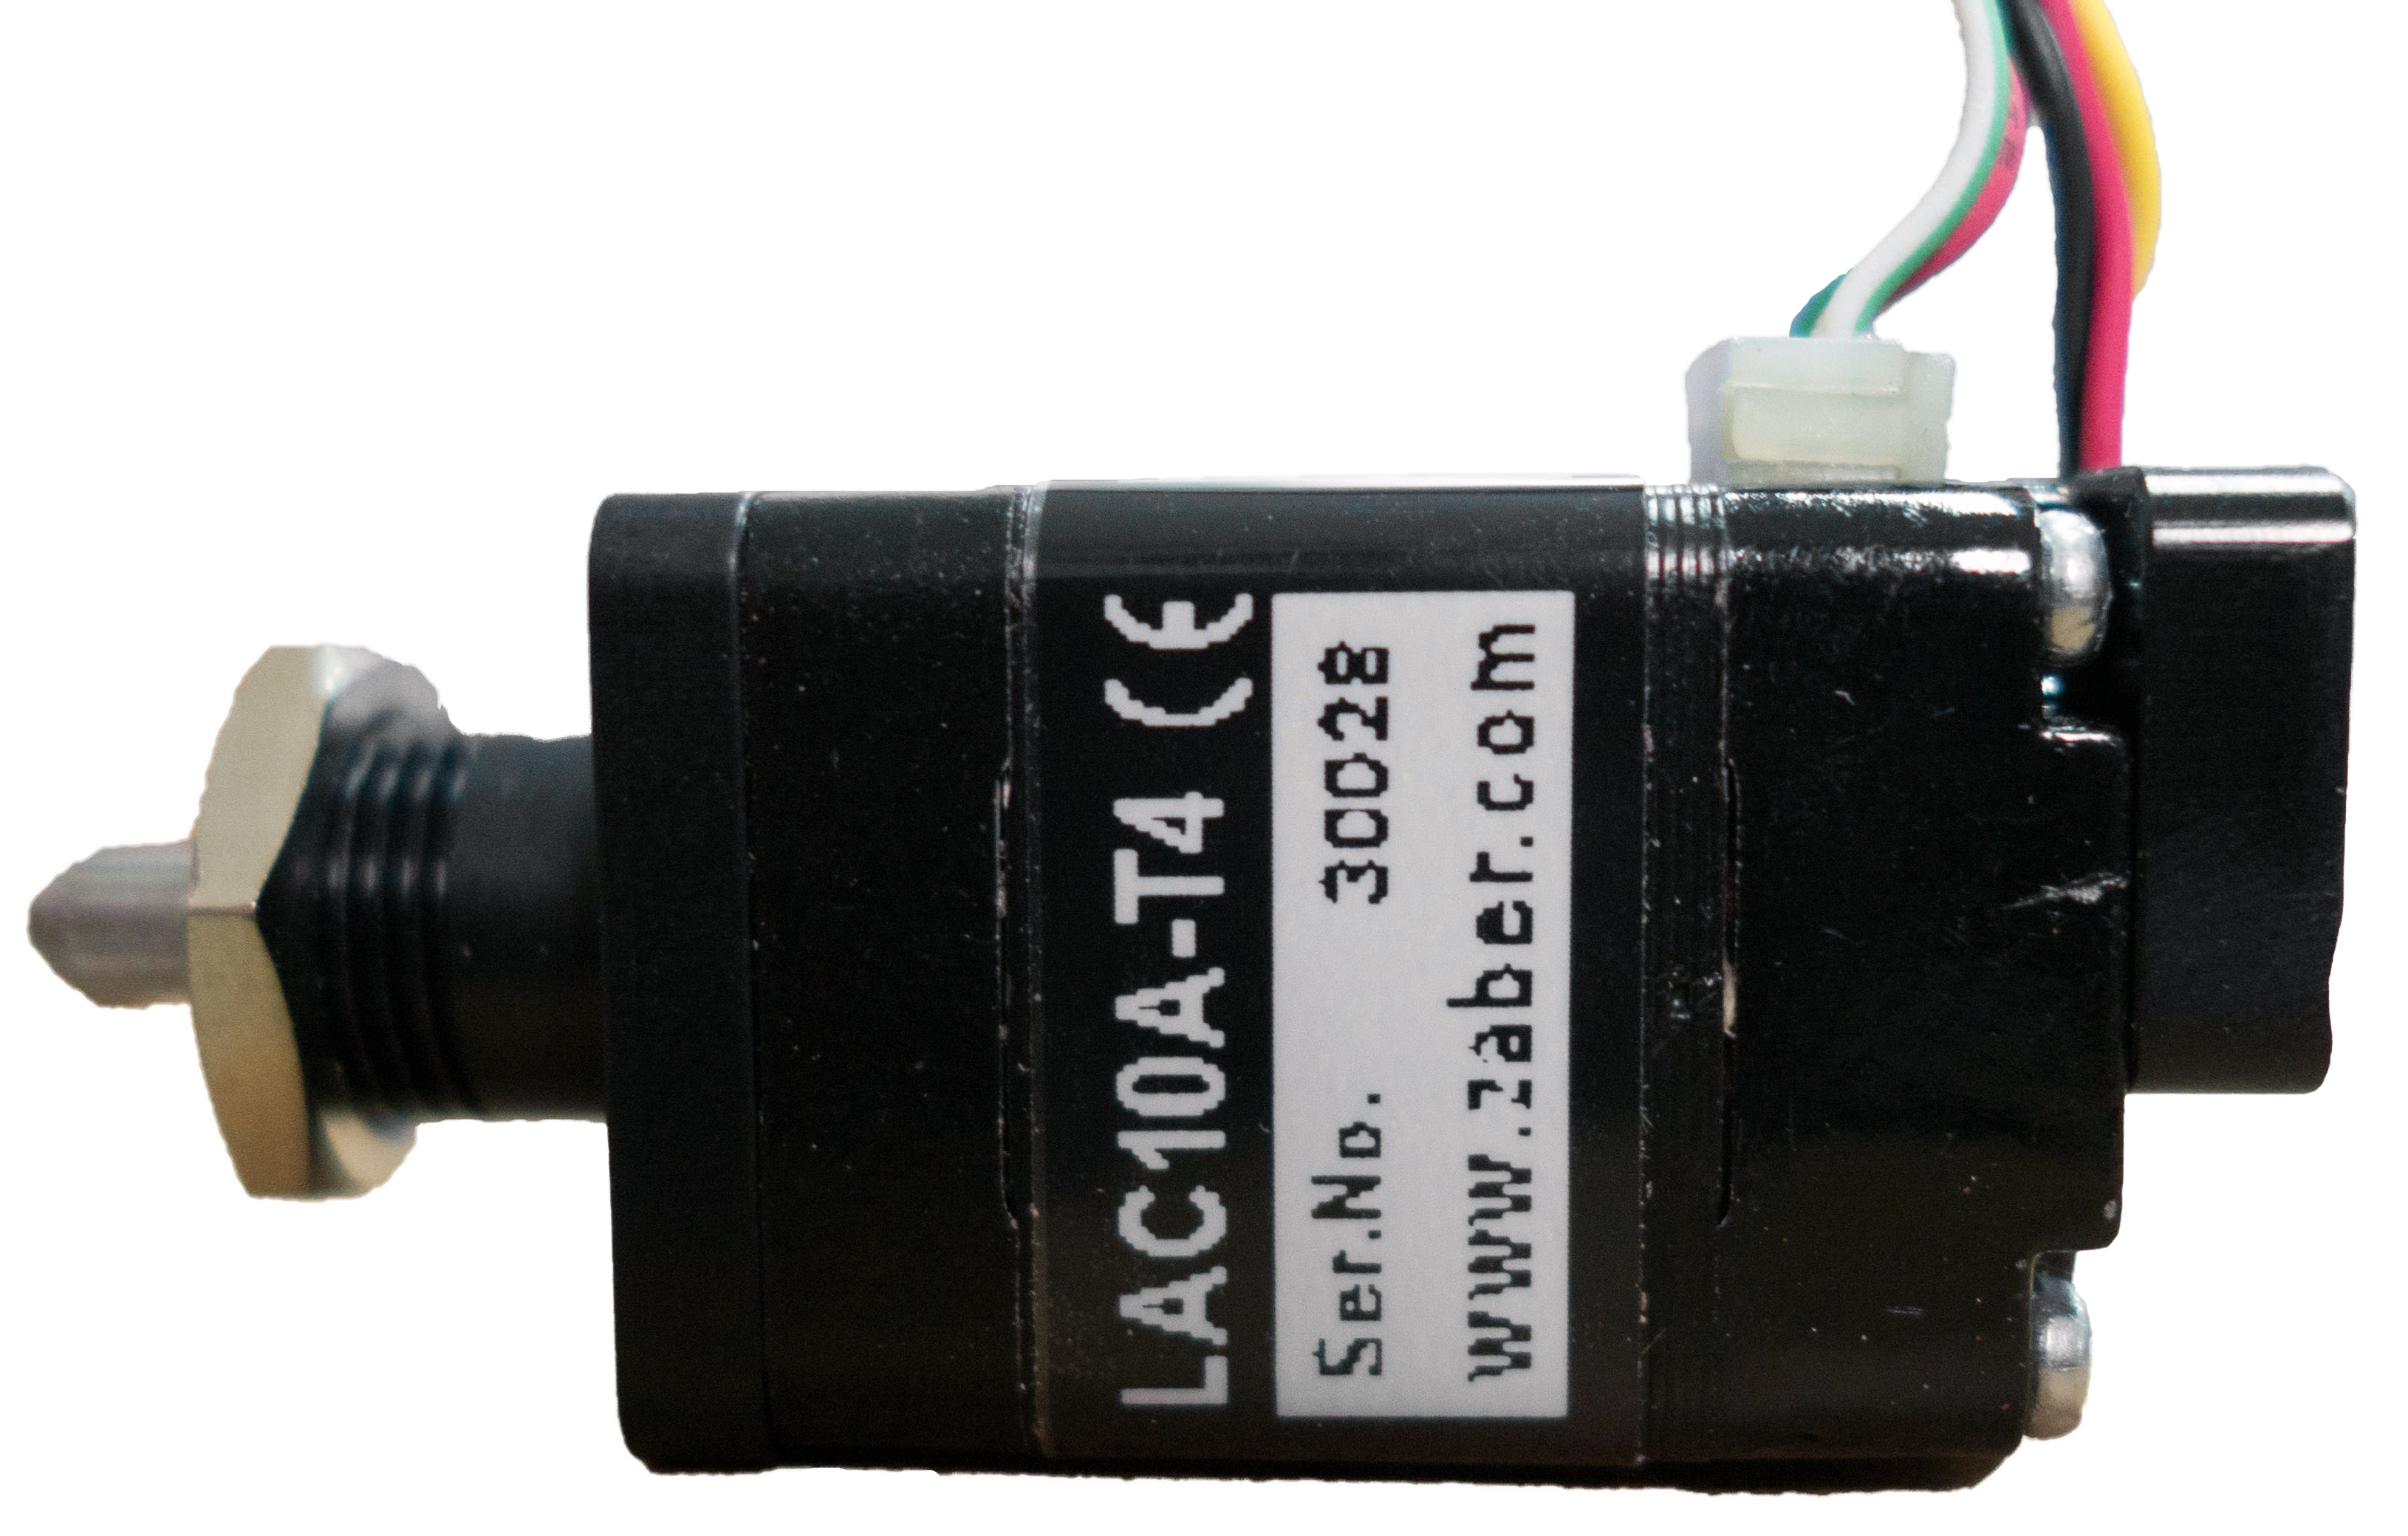
\includegraphics[width=0.618\linewidth]{rig/probe__feeding__LAC10A.png}
\caption{LAC10A-T4精密电动推杆}
\label{fig:rig-probe-feeding-LAC10A}
\end{figure}

\begin{figure}[tbh]
\centering
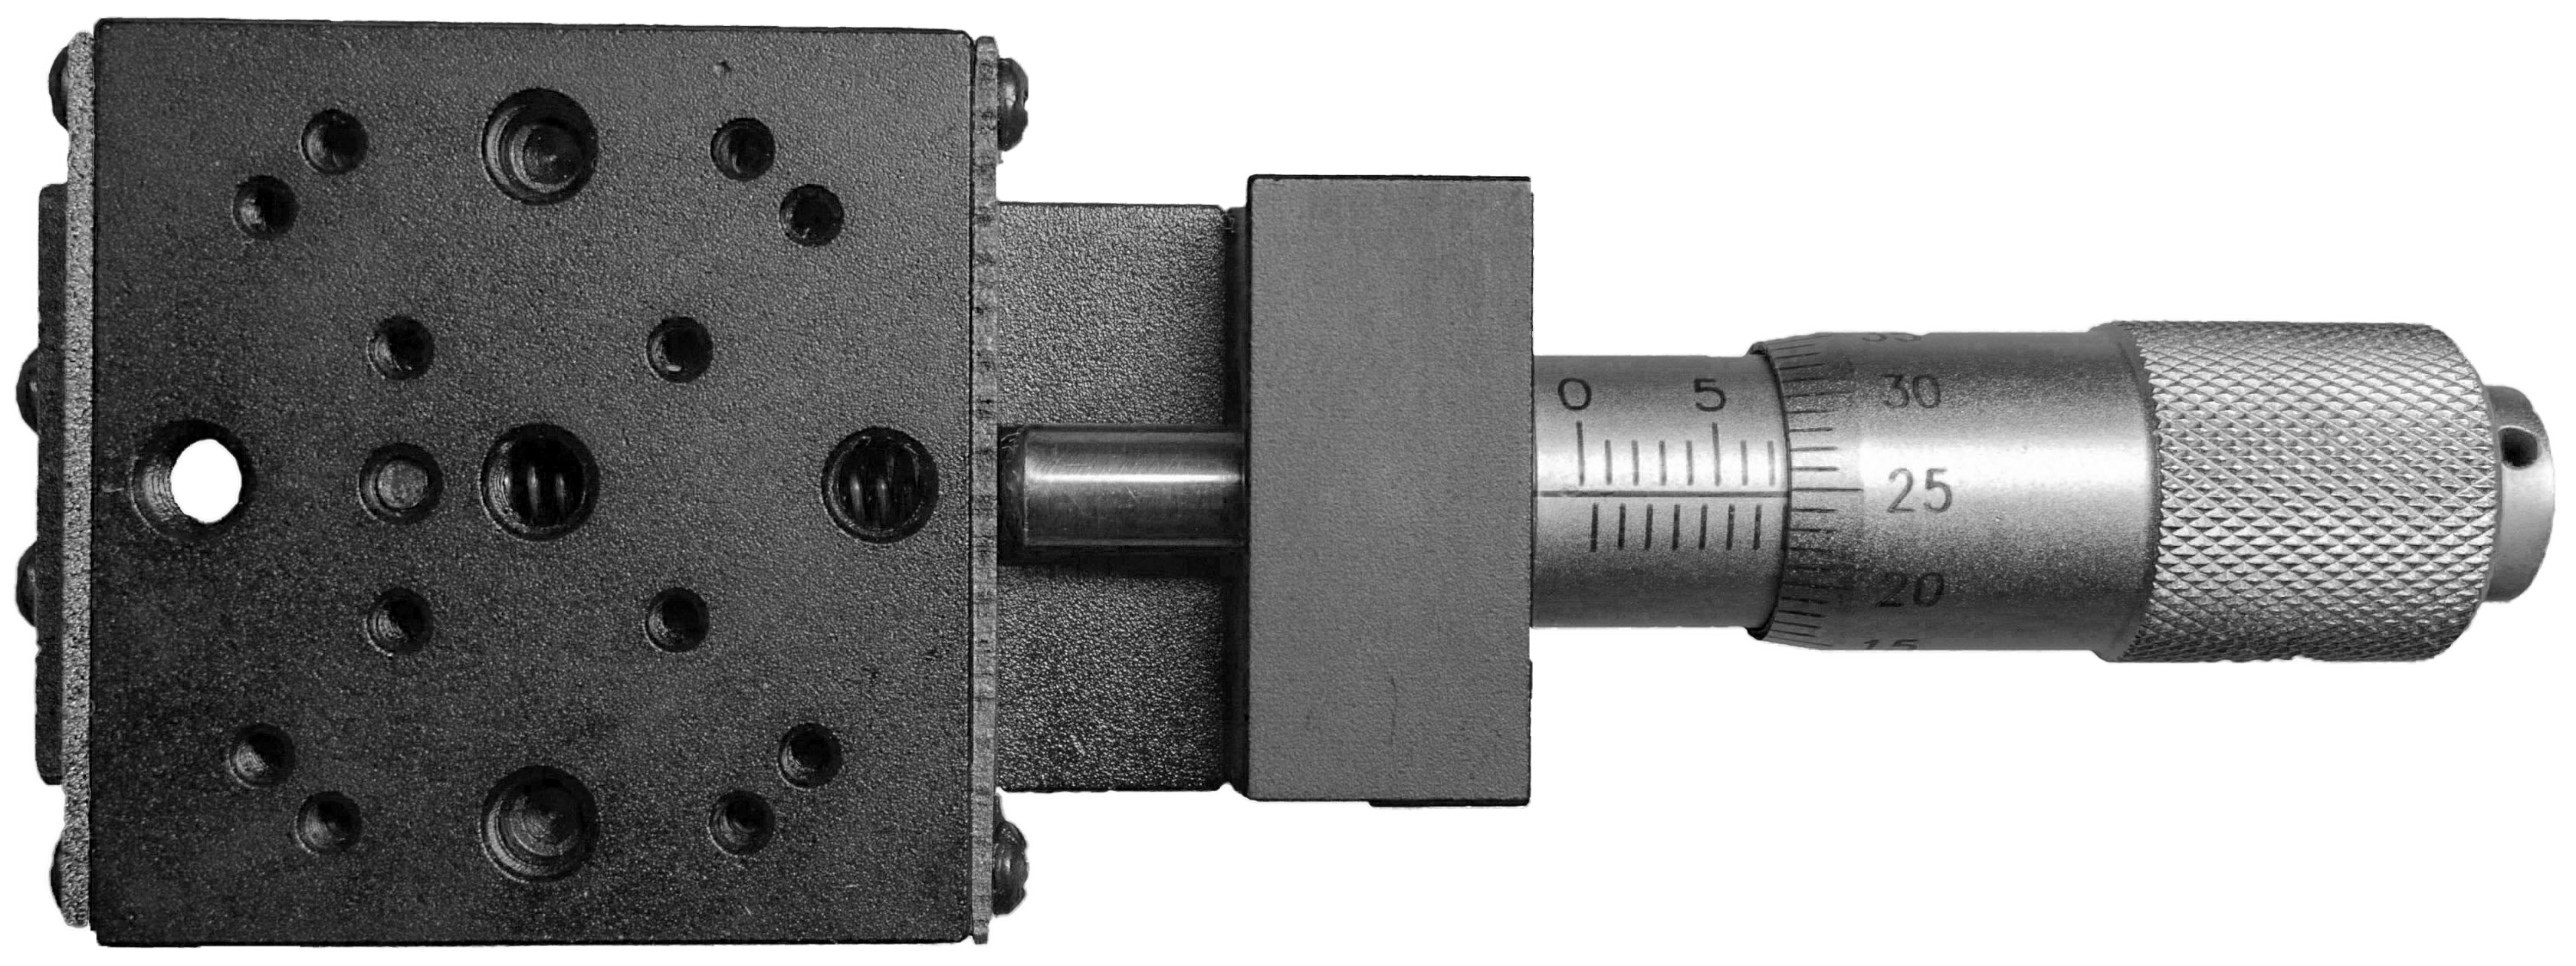
\includegraphics[width=0.618\linewidth]{rig/probe__feeding__JYPY.png}
\caption{JYPY-02213精密手动滑移台}
\label{fig:rig-probe-feeding-JYPY}
\end{figure}



\clearpage



\section{背吹控制系统设计}\label{sec:rig-pressure}

背吹平衡法需要控制静电卡盘背吹入口压强缓慢、平稳上升,并实时测量、记录该压强数值。如能同时测出进入背吹通道的流量,则可为之后的仿真分析提供更多数据参考。整个系统可分为供压与传感两部分,共同的关键参数为压强与流量。按照待测静电卡盘的参数($d = \SI{296}{\milli\meter}$,$F \leq \SI{200}{\newton}$)估算背吹入口压强最大值为\SI{5}{\kilo\pascal}\footnotemark{}。由于之前尚未有在大气环境下针对同尺寸的静电卡盘的背吹试验或仿真,流量范围未知,只能通过实测获得。本节将分别讨论供压、传感两部分的设计、工作原理与选型。
%then what is \ref{sec:principle-prob-flow-cfd-result}
%apparently it's invalid, but why?

\footnotetext{由于检测平台工作于大气环境下,所有涉及到的压强如无特殊说明均为表压(即相对于大气压强)。}


\subsection{供压方案分析}\label{sec:rig-pressure-supply}

普通气压控制元件(如减压过滤阀等)是为气动机械(如气缸、气爪、气动回转台等)设计的,输出压强下限一般为\SI{0.1}{\mega\pascal}级,超过上文估算的压强范围,因此需使用专用设备实现压强的精确控制。本节依次围绕集成电子压强控制单元、反馈控制微型气泵、以及精密机械式减压阀三个核心组件,提出对应的供压方案。由于影响供压系统性能因素较多,本节仅针对各方案做定性分析,需经实际搭建、测试验证方案可行性与性能。
%TODO:xref pressure impl

\subsubsection{集成电子压强控制单元}\label{sec:rig-pressure-supply-integrated}

这类产品集成了压强控制所需的所有电、气元件,接受一个电信号输入作为压强设定点,控制出口压强等于该设定点。其中,部分产品包括完整的显示、操作单元、通信接口等,如WIKA CPC2000/CPC6000压强控制器等(图~\ref{fig:rig-pressure-supply-cpc6000});部分产品只有简单的指示器,设定点为模拟信号(如$\SIrange{4}{20}{\milli\ampere}$信号),如TESCOM ER3000/ER5000系列、SMC ITV00x0系列电子比例阀等。完整的压强控制器较为昂贵,但精度较高,量程可选余地较大;电子比例阀成本较低,但其量程一般仍为气动机械级,而其中较小量程型号允许的流量较低(如SMC ITV0010型,最低输出压强\SI{1}{\kilo\pascal},最大流量仅\SI{3.5}{\liter\per\minute})。由于这类产品内部集成度较高,组成复杂,且订货周期较长,只能先通过数据手册标称值推测其性能,选取其中参数与供压系统要求匹配较好的产品订购,等待实际搭建验证。
%TODO:xref impl (ITV0010 epic fail, mention PQ already ordered)

\begin{figure}[tbh]
\centering
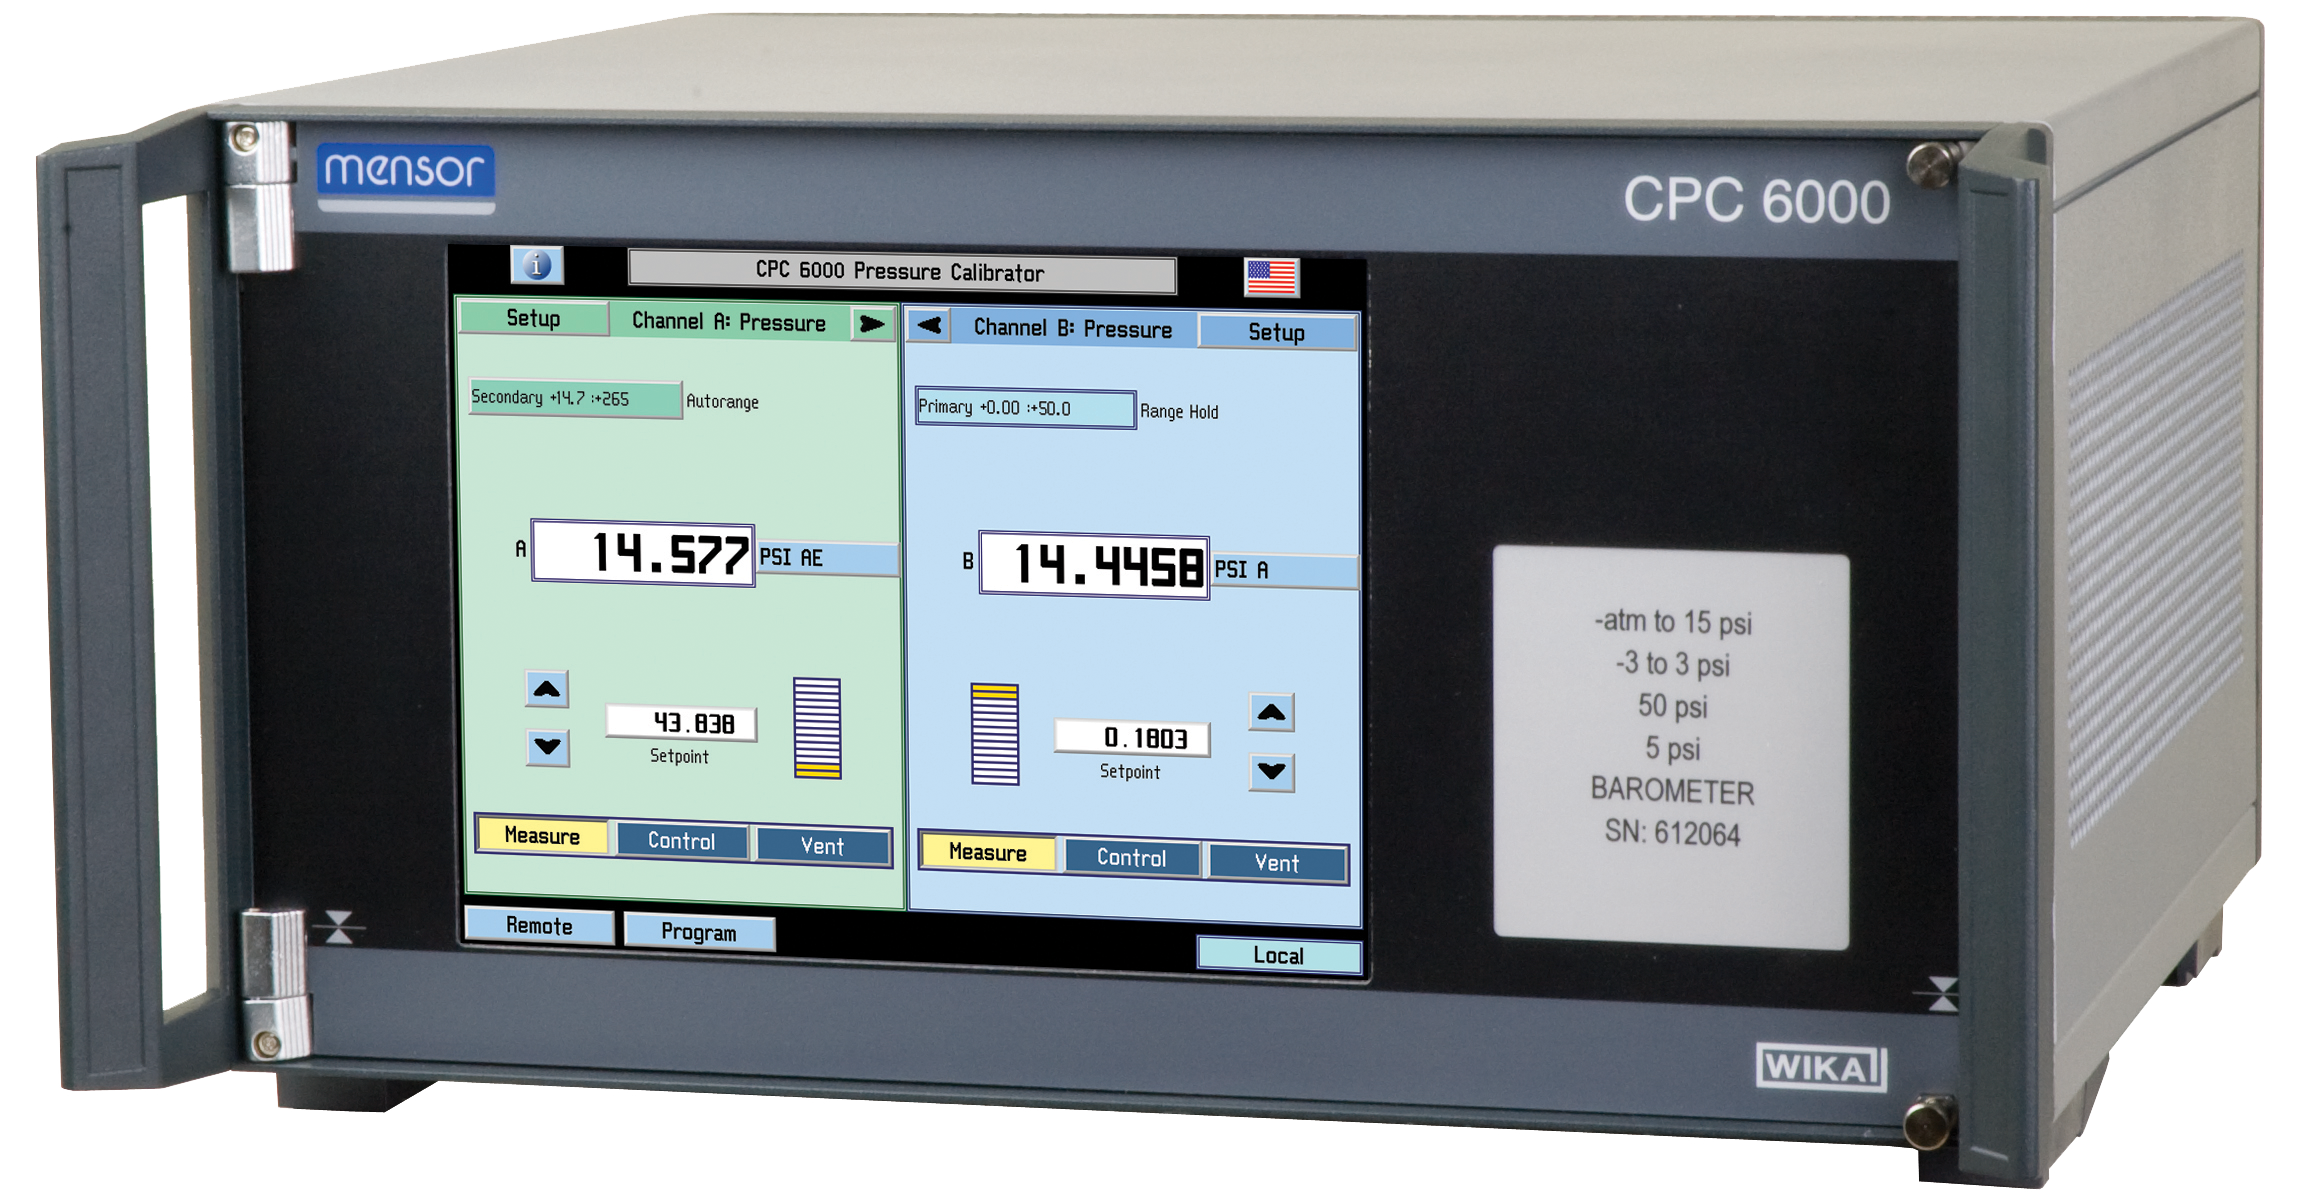
\includegraphics[width=0.75\linewidth]{rig/pressure__supply__cpc6000.png}
\caption{WIKA CPC6000压强控制器}
\label{fig:rig-pressure-supply-cpc6000}
\end{figure}

\subsubsection{反馈控制微型气泵}\label{sec:rig-pressure-supply-pump}

参考图~\ref{fig:rig-pressure-supply-cpc2000-sch},可用独立元件设计类似的压强控制系统,如图~\ref{fig:rig-pressure-supply-pump-sch}:使用直流电机驱动的微型气泵作为压力源,压强变送器提供反馈信号,闭环PI控制气泵输出功率。为减小气泵固有的压强波动,可采取如下措施:

\begin{enumerate}
  \item 在泵与背吹通道入口间增设双端气瓶,通过增加惯性环节的方式降低压强波动;
  \item 在背吹通道入口处加设一节流阀通向大气,避免电机反复启停造成的压强波动;
\end{enumerate}

\begin{figure}[tbh]
\centering
\includegraphics[width=1\linewidth]{rig/pressure__supply__cpc2000__sch.png}
\caption{CPC2000工作原理示意}
\label{fig:rig-pressure-supply-cpc2000-sch}
\end{figure}

\begin{figure}[tbhp]
\centering
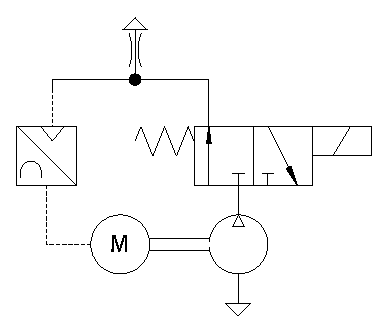
\includegraphics[width=0.5\linewidth]{rig/pressure__supply__pump__sch}
\caption{反馈控制微型气泵示意}
\label{fig:rig-pressure-supply-pump-sch}
\end{figure}

\subsubsection{精密机械式减压阀}\label{sec:rig-pressure-supply-reg}

机械式减压阀的基本原理是:入口与出口间有一开度可调的小孔,其开度由出口压强通过膜片负反馈控制,从而维持出口压强恒定。根据其具体结构不同,部分机械式减压阀在小孔开度接近0时,出口压强可低于其标称最低输出压强,但不能起到稳压作用(即出口压强与流量相关)。如SMC IR1000型精密减压阀(图~\ref{fig:rig-pressure-supply-ir1000}),标称调压范围$\SIrange{5}{200}{\kilo\pascal}$,标称灵敏度\SI{0.4}{\kilo\pascal}。该产品调压范围可满足\ref{sec:rig-pressure-supply-integrated}节中提到的电子比例阀的入口压强范围要求,因此可作为其前置减压阀使用。同时,虽然其标称最低输出压强大于供压系统最大输出压强,但考虑其工作原理(具有静态放气通路)允许其出口压强低于标称最低输出压强,可以尝试将其出口直接连接背吹入口,用于提供$\SIrange{0}{5}{\kilo\pascal}$范围内的缓慢变化的压强。
%TODO:xref impl (manual IR1000 works)

\begin{figure}[tbhp]
\centering
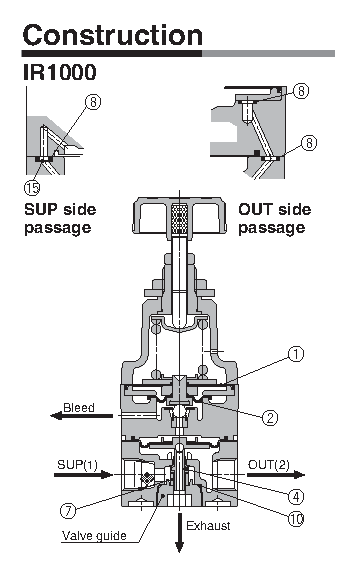
\includegraphics[height=0.55\textheight]{rig/pressure__supply__IR1000}
\caption{IR1000简化剖视}
\label{fig:rig-pressure-supply-ir1000}
\end{figure}


\subsection{传感部分选型}\label{sec:rig-pressure-sensor}

无论供压部分采用何种方案,均不影响压强传感器的选型。完整的选型表见附录B。
%TODO:xref appendix (pressure mashup)
最终选定Honeywell STD720精密差压变送器(量程可在$\pm \num{1} \sim \pm \SI{100}{\kilo\pascal}$范围内任意配置,基础准确度$0.05\%$,输出$\SIrange{4}{20}{\milli\ampere}$模拟信号、HART现场总线协议)。另外配置\SI{16}{\kilo\pascal}量程的机械指针式压强计,辅助调试。


\subsection{过压保护措施}\label{sec:rig-pressure-valve}

由\ref{principle-soln-ruby}节\eqref{eq:principle-soln-ruby-force}式知,晶圆脱附后,微力探头受的压缩力随背吹气压升高而升高,若传感器受力突增至超过其安全过载范围,则有对传感器造成不可恢复的损伤的风险。因此在气路中加入两位三通电磁阀:通电时系统接通压力源,背吹通道压强正常;断电时系统通向大气,背吹通道无压强。在检测过程中,时刻监测传感器受力,一旦超过事先设定的警戒线,立即切断气压,从而避免传感器受损。



\clearpage



\section{机械结构设计}\label{sec:rig-model}

根据图~\ref{fig:rig-overall-sch},设计测试平台的机械结构。为了方便加工、搭建,选用标准$\num{30} \times \SI{30}{\milli\meter}$系列开槽铝合金型材及配套标准连接件,与依据待测静电卡盘的外形尺寸设计的连接板共同构成框架结构;其他组件均通过连接件与之相连。框架结构的简化三维模型如图~\ref{fig:rig-model-all-iso}\footnote{型材连接部分零件数较多,因此并未全部在总装配体三维模型中表示出。}。

\begin{figure}[p]
\centering
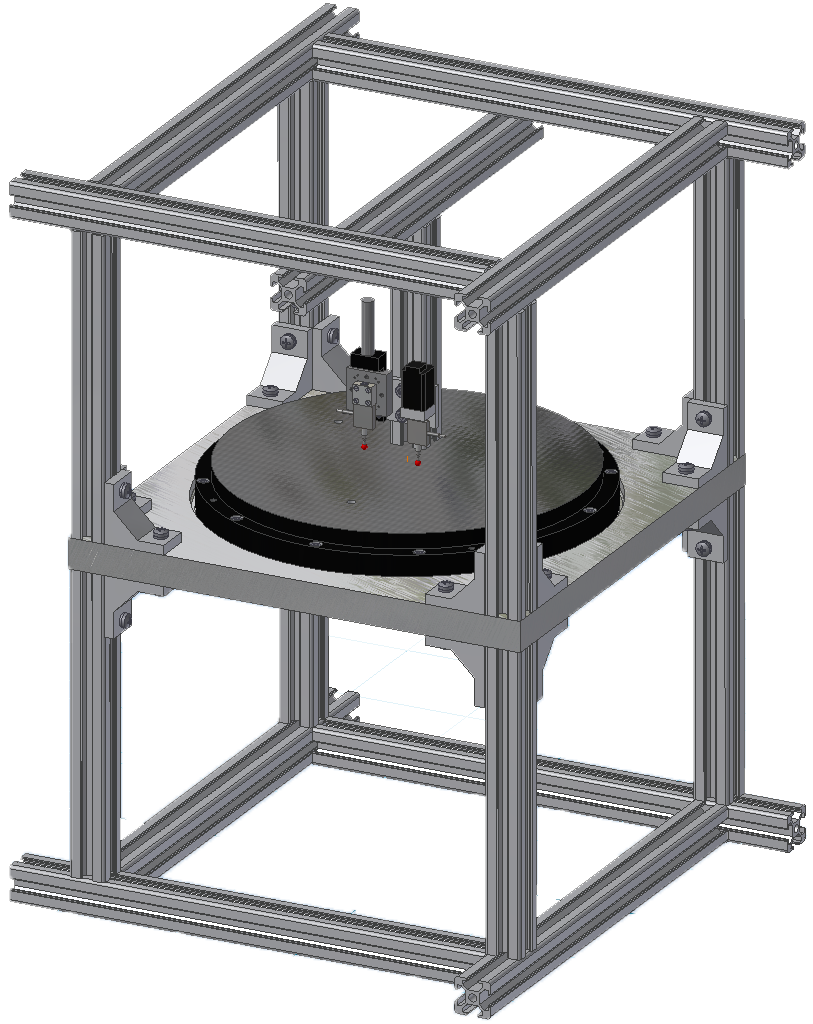
\includegraphics[width=1\textwidth]{rig/model__all__iso.png}
\caption{测试平台装配体三维模型}
\label{fig:rig-model-all-iso}
\end{figure}


\subsection{静电卡盘连接板}\label{sec:rig-model-base}

该连接板位于整个测试平台中心,其尺寸与配合特征主要由静电卡盘决定,并间接决定了整个框架的尺寸。静电卡盘通过螺钉紧固在连接板上,因此连接板需提供相配合的螺纹孔与承载面。如图~\ref{fig:rig-model-echuck-back}\footnotemark{},静电卡盘的底部有多个功能特征,除氦气背吹接口需特殊设计外,其他特征(如直流电极接口、顶针孔等)均需裸露在外以正常使用,因此连接板上对应位置开槽。背吹通道入口并未采用常见的螺纹连接方式,而是一$\diameter{}4$光孔,需设计密封接头与之相连。如图~\ref{fig:rig-model-echuck-plug-assy},用三个紧定螺钉使密封接头上表面与卡盘背面紧密配合,通过标准O型圈形成端面密封;其另一端提供M5内螺纹,与标准气动快装接头连接。

\footnotetext{北方微电子公司内部图纸,仅保留轮廓与功能描述。}

\begin{figure}[tbhp]
\centering
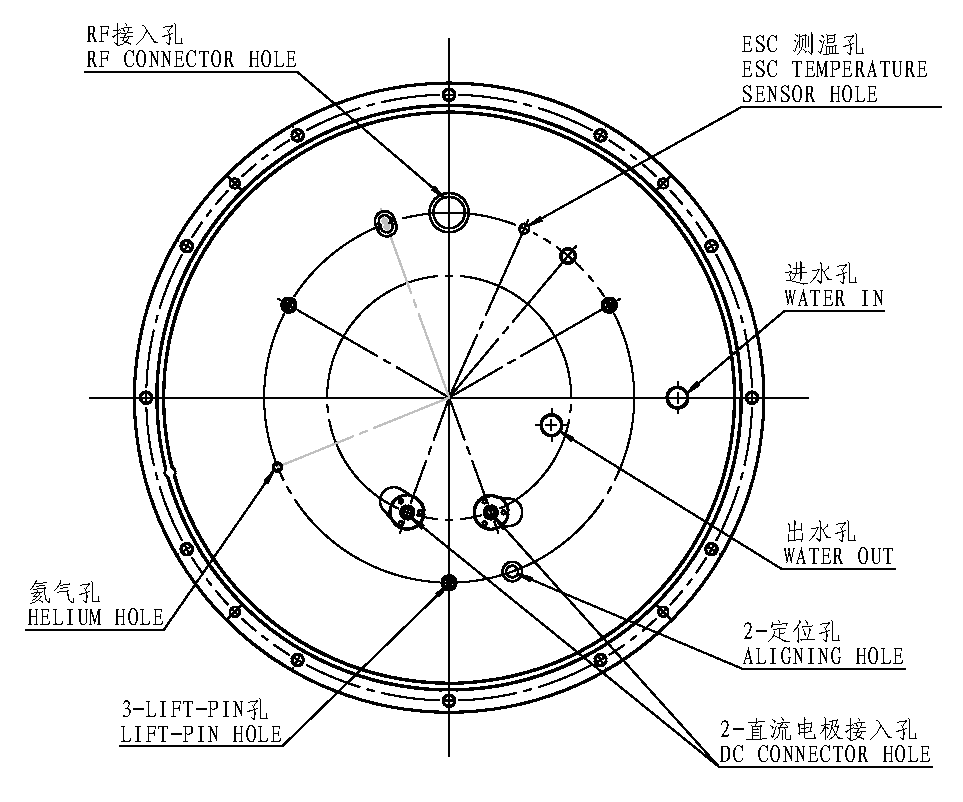
\includegraphics[height=0.45\textheight]{rig/model__echuck__back}
\caption{静电卡盘背面特征工程图}
\label{fig:rig-model-echuck-back}
\end{figure}

\begin{figure}[tbhp]
\centering
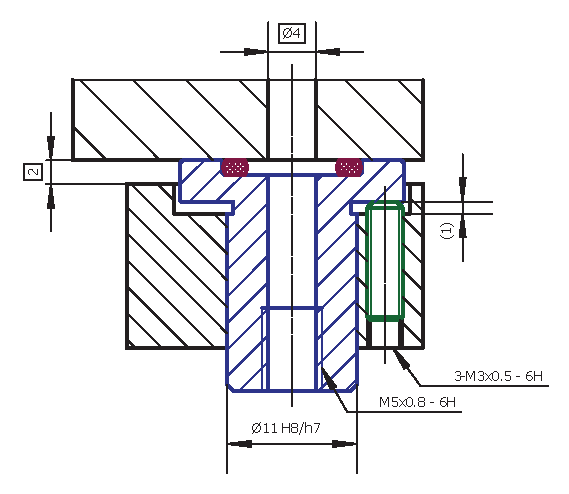
\includegraphics[height=0.45\textheight]{rig/model__echuck__plug__assy2}
\caption{端面密封设计工程图}
\label{fig:rig-model-echuck-plug-assy}
\end{figure}


\subsection{型材框架主体}\label{sec:rig-model-frame}

框架主体设计为三层对称结构:中间一层是静电卡盘连接板,上下两层均为4根型材用铸钢角件和紧定螺钉连接成的正方形结构;层与层之间用4根纵向型材负责承重,在连接板侧使用$\num{50}\times\num{50}\times\SI{30}{\milli\meter}$挤压角件连接(三维模型中已表示出),在正方形框架侧使用$\num{60}\times\num{60}\times\SI{30}{\milli\meter}$角件连接。这种连接方式的主要优点是不依靠型材与角件的摩擦力承受重量,而是靠型材、角件、连接螺栓将载荷传至地面,稳定可靠。


\subsection{微力探头部分}\label{sec:rig-model-probe}

由于红宝石探头的连接螺纹为M2外螺纹,LSB200的连接螺纹为M3内螺纹,设计螺纹转接头如图~\ref{fig:rig-model-probe-connLSBRuby}。由\ref{sec:rig-probe-feeding}节中讨论,需设计微力探头组件位置粗调结构。考虑到LAC-10A电动推杆的行程为\SI{10}{\milli\meter},采用最简单易行的设计(三维模型中已表示出):在框架结构上部加装可自由调节位置的型材组,由横、竖两根型材构成;横梁用螺栓、大垫圈、T槽螺母连接在框架上层四边形的下面;竖梁使用$\num{60}\times\num{60}\times\SI{30}{\milli\meter}$角件与横梁连接。在此基础上,设计微力探头组件连接板如图~\ref{fig:rig-model-probe-connBridgeProbesMain};连接板与LAC-10A通过图~\ref{fig:rig-model-probe-connBridgeProbesTab}所示连接 块、沉头螺钉相连,与JYPY-02213通过沉头螺钉相连。连接板本身可通过螺栓与T槽螺母可紧固在竖梁任意位置。这样即可手动大范围调节微力探头在空间中的位置。
这一部分整体三维模型如图~\ref{fig:rig-model-probe};其中两组微力探头是为了同时在图中表示探头与LAC-10A和JYPY-02213的连接方式,实际仅选装一组。

%TODO:conn JYPY LSB

\begin{figure}[tbh]
\centering
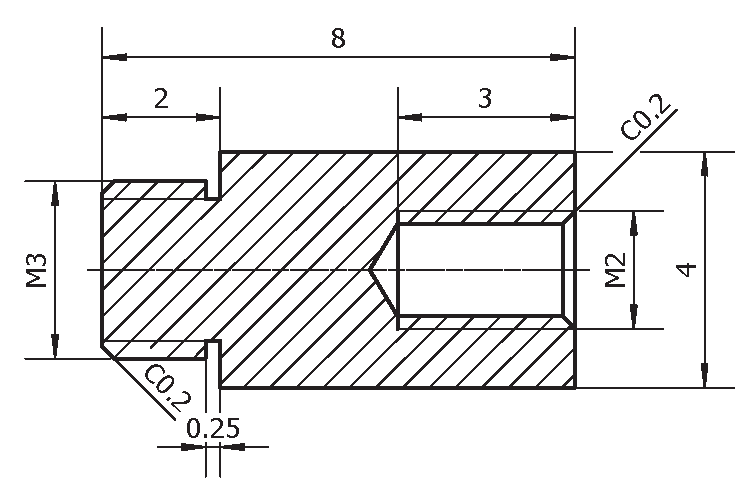
\includegraphics[width=0.6\linewidth]{rig/model__probe__connLSBRuby}
\caption{M2$\to$M3 螺纹转接头零件图}
\label{fig:rig-model-probe-connLSBRuby}
\end{figure}

\begin{figure}[tbh]
\centering
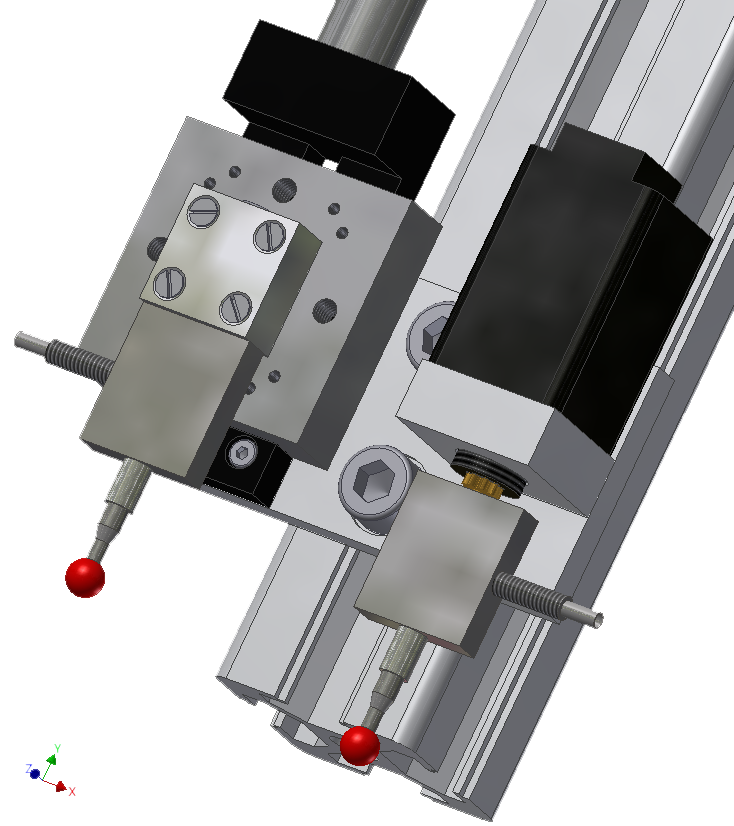
\includegraphics[height=0.40\textheight]{rig/model__probe.png}
\caption{探头组件数字模型}
\label{fig:rig-model-probe}
\end{figure}

\begin{figure}[p]
\centering
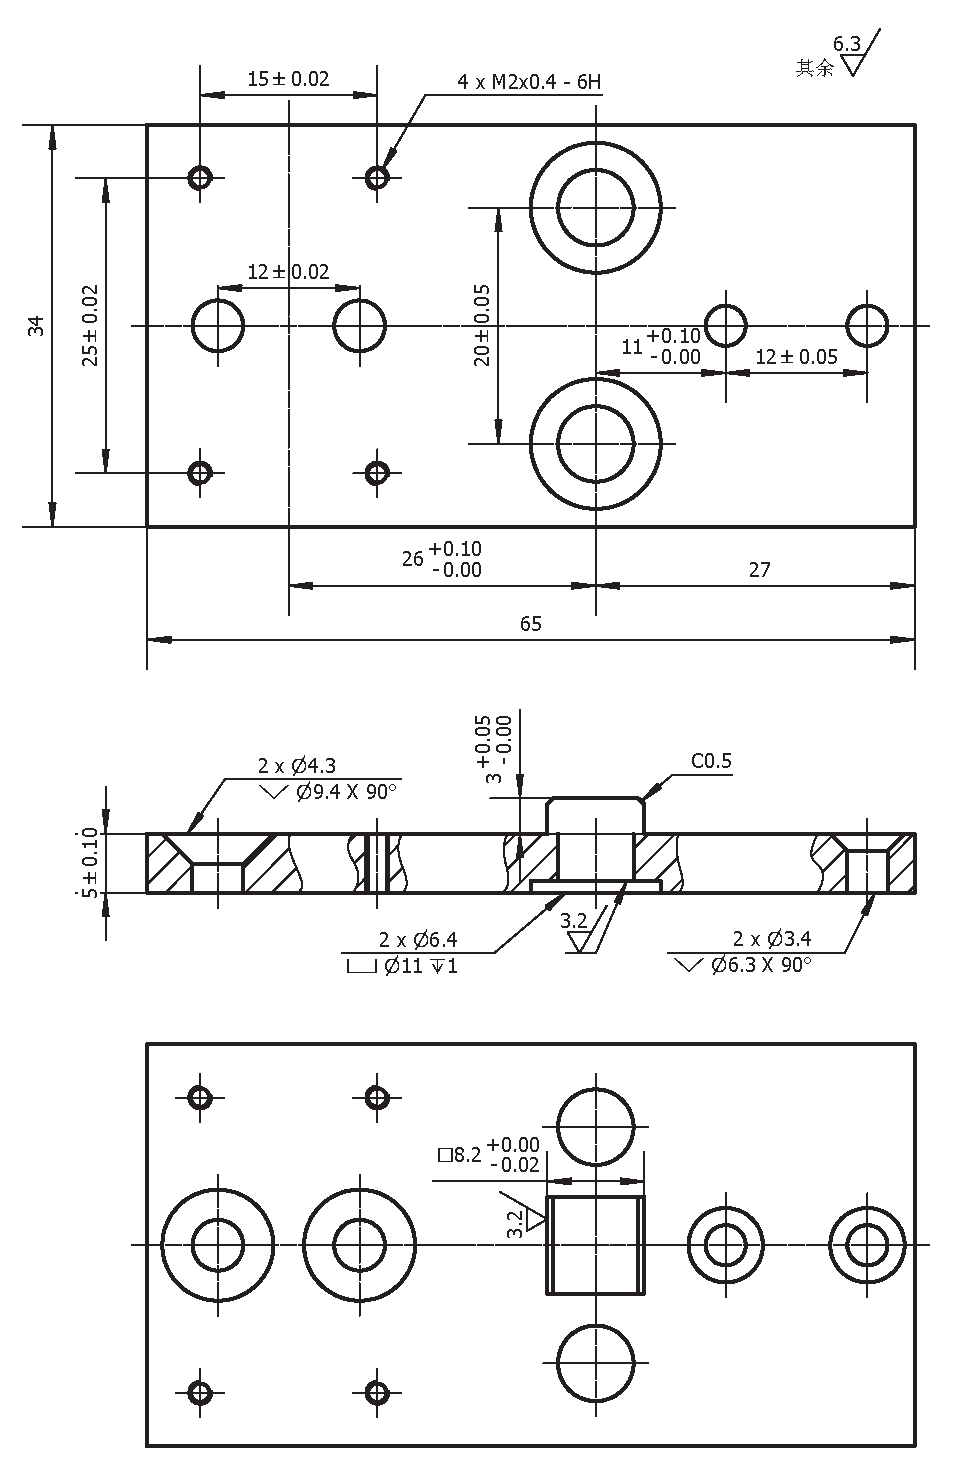
\includegraphics[height=1\textheight]{rig/model__probe__connBridgeProbesMain}
\caption{微力探头组件连接板零件图}
\label{fig:rig-model-probe-connBridgeProbesMain}
\end{figure}

\begin{figure}[p]
\centering
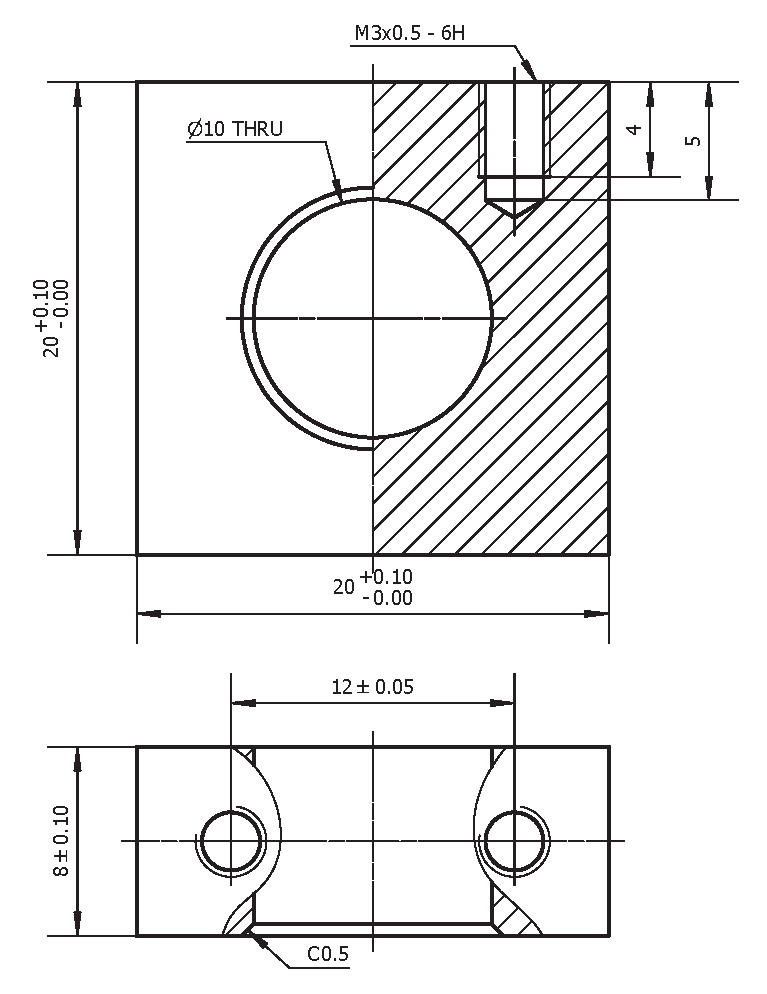
\includegraphics[height=0.48\textheight]{rig/model__probe__connBridgeProbesTab}
\caption{LAC-10A连接块零件图}
\label{fig:rig-model-probe-connBridgeProbesTab}
\end{figure}

\begin{figure}[p]
\centering
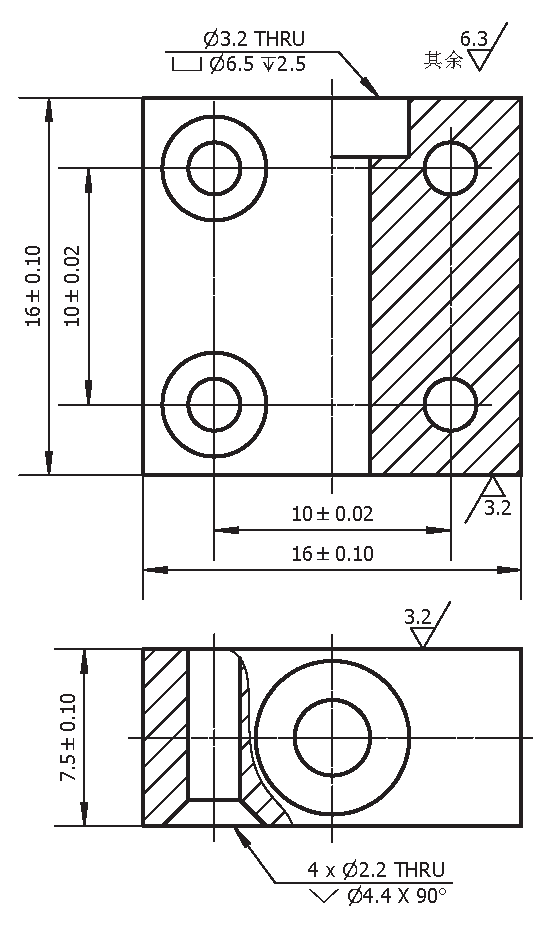
\includegraphics[height=0.42\textheight]{rig/model__probe__connJYPYLSB}
\caption{JYPY-02213连接块零件图}
\label{fig:rig-model-probe-connJYPYLSB}
\end{figure}





\clearpage



\section{自动控制与数据采集系统设计}\label{sec:rig-ctrl}

由于检测平台中存在多种输入输出信号类型各异的电子传感/执行模块,且部分控制对实时性要求高,因此以微控制器单元(MCU)为核心设计自动控制与数据采集系统(下文简称“电控系统”);其组成以及各组件间信号流动关系如图~\ref{fig:rig-ctrl-sch}。可将电控系统分为四个层次,自底向上分别为:传感/执行模块、接口电路、MCU、PC。传感/执行模块即检测平台中使用的压强变送器、电子比例阀、微力传感器等元件。这些模块分散在检测平台各处,接受的输入/输出信号类型各异,需通过匹配的接口电路进行信号处理、转换、隔离等,统一为3.3V电压的数字(包括总线)与模拟信号,再连接到MCU上。本节首先重点针对各传感/执行模块,设计匹配其特性、满足检测平台使用需要的接口电路;然后根据接口电路特点与检测需求,讨论MCU部分的软硬件设计。PC部分主要负责MCU和智能仪表(见\ref{sec:rig-ctrl-intf-loop}节)通信,对其发送指令,接受其回传的数据;这些功能均可使用现有软件完成,不在电控系统具体设计范畴,本节不再讨论。

\begin{figure}[h]
\centering
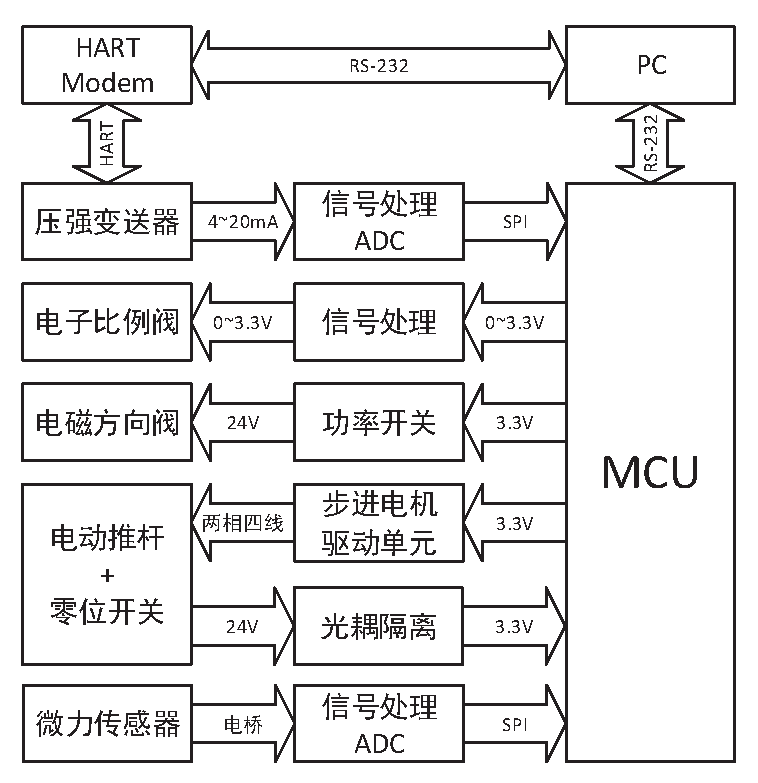
\includegraphics[height=0.5\textheight]{rig/ctrl__sch}
\caption{电控系统组成}
\label{fig:rig-ctrl-sch}
\end{figure}



\subsection{压强变送器接口}\label{sec:rig-ctrl-intf-loop}

\ref{sec:rig-pressure-sensor}节选择的Honeywell STD720精密差压变送器属于Honeywell SmartLine智能数字仪表系列,内置数字信号处理器,为单电源+24V供电的2线制\SIrange{4}{20}{\milli\ampere}电流环变送器设备,并支持HART现场总线协议。虽然可以通过HART协议直接从仪表读取压强数值,由于HART传输速率非常低,一个完整的请求 -- 应答过程可耗时\SI{0.25}{\second}以上,与变送器本身的\SI{50}{\hertz}采样率严重不匹配,因此HART协议仅供仪表配置与标定使用,通过独立的HART Modem与PC连接,并使用Honeywell官方提供的软件对其进行配置,而压强的实时数值从\SIrange{4}{20}{\milli\ampere}电流环获取。

接口电路总体构成如图~\ref{fig:rig-ctrl-intf-loop-sch-root}:将电流信号转换为电压信号后,接入ADC转换为数字量,由MCU通过SPI串行总线读取。模拟前端(信号转换与处理)部分如图~\ref{fig:rig-ctrl-intf-loop-sch-sample}:稳压滤波过的+24V电压接入变送器正极接线柱(+)为其供电,变送器负极接线柱(-)输出的\SIrange{4}{20}{\milli\ampere}电流信号经过\SI{240}{\ohm}采样电阻R2得到\SIrange{0.96}{4.8}{\milli\volt}电压信号,经R3、C1一阶滤波,接入ADC模拟输入端。这里R1起双重作用:与C6组成电源滤波器(并非唯一,见\ref{sec:impl-pcb-pressure}中供电部分),使电流环中串联电阻(R1、R2)不低于\SI{250}{\ohm}以满足HART协议物理层要求。ADC选用AD768x系列\footnotemark{},可直接使用对应数据手册中参考电路,具体实现不再赘述。

\footnotetext{ADI公司AD768x系列、TI公司ADS888x系列为针脚、封装均兼容,功能相同,但性能参数各异的SPI接口SAR(连续逼近)型ADC,由于从ADI公司获取了AD7686样片,下文中该ADC统一称为``AD7686''。}

\begin{figure}[tb]
\centering
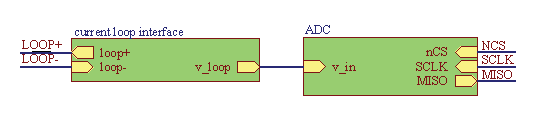
\includegraphics[width=0.8\linewidth]{rig/ctrl__intf__loop__sch__root}
\caption{\SIrange{4}{20}{\milli\ampere}电流环接口电路原理图(总体)}
\label{fig:rig-ctrl-intf-loop-sch-root}
\end{figure}

\begin{figure}[tb]
\centering
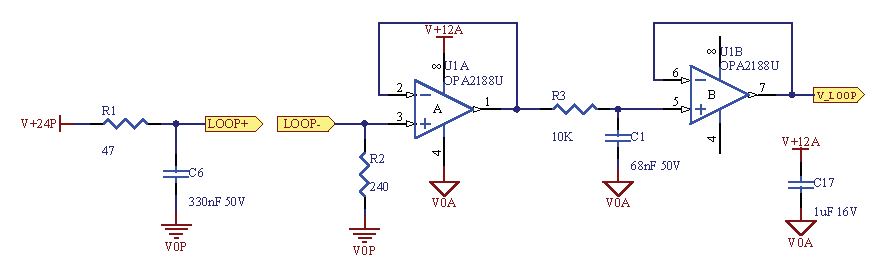
\includegraphics[width=1\linewidth]{rig/ctrl__intf__loop__sch__sample}
\caption{\SIrange{4}{20}{\milli\ampere}电流环接口电路原理图(前端)}
\label{fig:rig-ctrl-intf-loop-sch-sample}
\end{figure}

\subsection{电子比例阀接口}\label{sec:rig-ctrl-intf-reg}

\ref{sec:rig-pressure-supply-integrated}节中提到的压力控制器或电子比例阀接受的设定点输入分为两种:模拟电压信号、\SIrange{4}{20}{\milli\ampere}模拟电流环信号。模拟电压输入可直接通过单片机内置DAC(输出范围\SIrange{0}{3.3}{\volt})经一级放大滤波得到,其原理图与图\ref{fig:rig-ctrl-intf-loop-sch-sample}中采样电阻之后的部分基本相同,不再赘述。模拟电流输入可用AD420集成电流输出DAC提供,接法如图~\ref{fig:rig-ctrl-intf-ad420}。

\begin{figure}[tbhp]
\centering
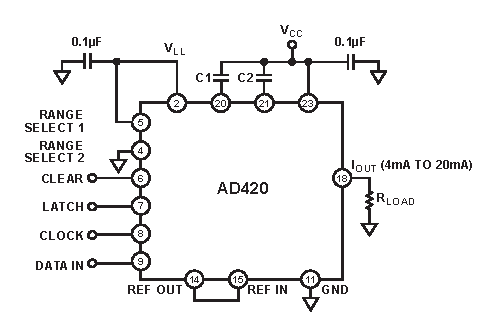
\includegraphics[width=0.618\linewidth]{rig/ctrl__intf__ad420}
\caption{AD420接法原理图}
\label{fig:rig-ctrl-intf-ad420}
\end{figure}

\subsection{电磁方向阀接口}\label{sec:rig-ctrl-intf-relay}

\ref{sec:rig-pressure-valve}节中的电磁方向阀(两位三通)在电路中等效为一直流\SI{24}{\volt}继电器,可使用常见的ULN2003集成功率开关驱动,如图~\ref{fig:rig-ctrl-intf-uln2003}。由于ULN2003内置续流二极管,输出端无需任何被动元件;R14为输入端下拉电阻,防止输入悬空时受电磁干扰产生误动作。

\begin{figure}[tbhp]
\centering
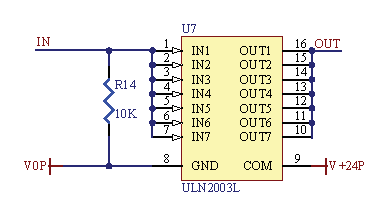
\includegraphics[width=0.618\linewidth]{rig/ctrl__intf__uln2003}
\caption{ULN2003功率开关原理图}
\label{fig:rig-ctrl-intf-uln2003}
\end{figure}

\subsection{电动推杆接口}\label{sec:rig-ctrl-intf-stepper}

\ref{sec:rig-probe-feeding}节中选择的LAC-10A电动推杆使用两相四线混合式步进电机作为驱动力,并使用永磁铁 -- 霍尔开关作为零位传感器。该步进电机的相电阻较高,为\SI{20.4}{\ohm},而额定电流较低,为\SI{0.24}{\ampere},需要使用与之相匹配的步进电机驱动器。最终选择雷赛DM422C数字式步进电机驱动器,其输出峰值电流可事先以\SI{0.1}{\ampere}为单位通过串口配置,通过2片MAX490E差分输入输出接口芯片(图~\ref{fig:rig-ctrl-intf-max490e})分别接收MCU发出的脉冲、方向指令信号。

LAC-10A附带的零位传感器使用标准的3线开漏(open drain)输出霍尔开关A1122:平时输出悬空;当在电动推杆即将到达其最短位置时,磁铁靠近霍尔开关,使其动作,输出被下拉至地;由于霍尔开关具有滞回(hysterisis),此时只有电动推杆向伸长方向移动一小段确定的距离后,输出才会恢复悬空状态。由于电机附近存在较强电磁干扰,为避免因此产生误动作,可增加霍尔开关供电电压至\SIrange{12}{24}{\volt}\footnotemark{},通过光耦隔离,转换为\SI{3.3}{\volt}信号,如图~\ref{fig:rig-ctrl-intf-opto}:U2为普通光耦,R1为光耦输入端串联限流电阻,输出端R2为上拉电阻。零位传感器等效为开关J1,平时J1断开,\bverb|out|为高电平(\SI{3.3}{\volt});动作时J1闭合,U2接通,\bverb|out|为低电平(0);该信号即可直接接入MCU。

\footnotetext{A1122数据手册中标称\SI{24}{\volt}为最大供给电压,因此实际供给电压应 严格小于\SI{24}{\volt}。}

\begin{figure}[p]
\centering
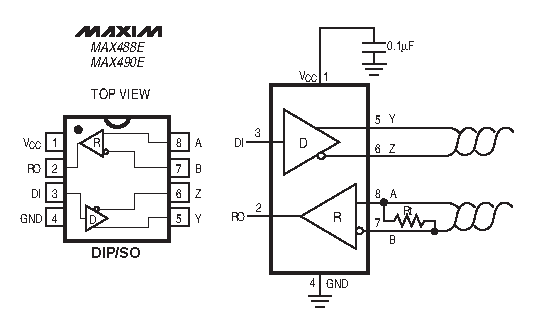
\includegraphics[width=0.7\linewidth]{rig/ctrl__intf__max490e}
\caption{MAX490E差分输入输出原理图}
\label{fig:rig-ctrl-intf-max490e}
\end{figure}

\begin{figure}[p]
\centering
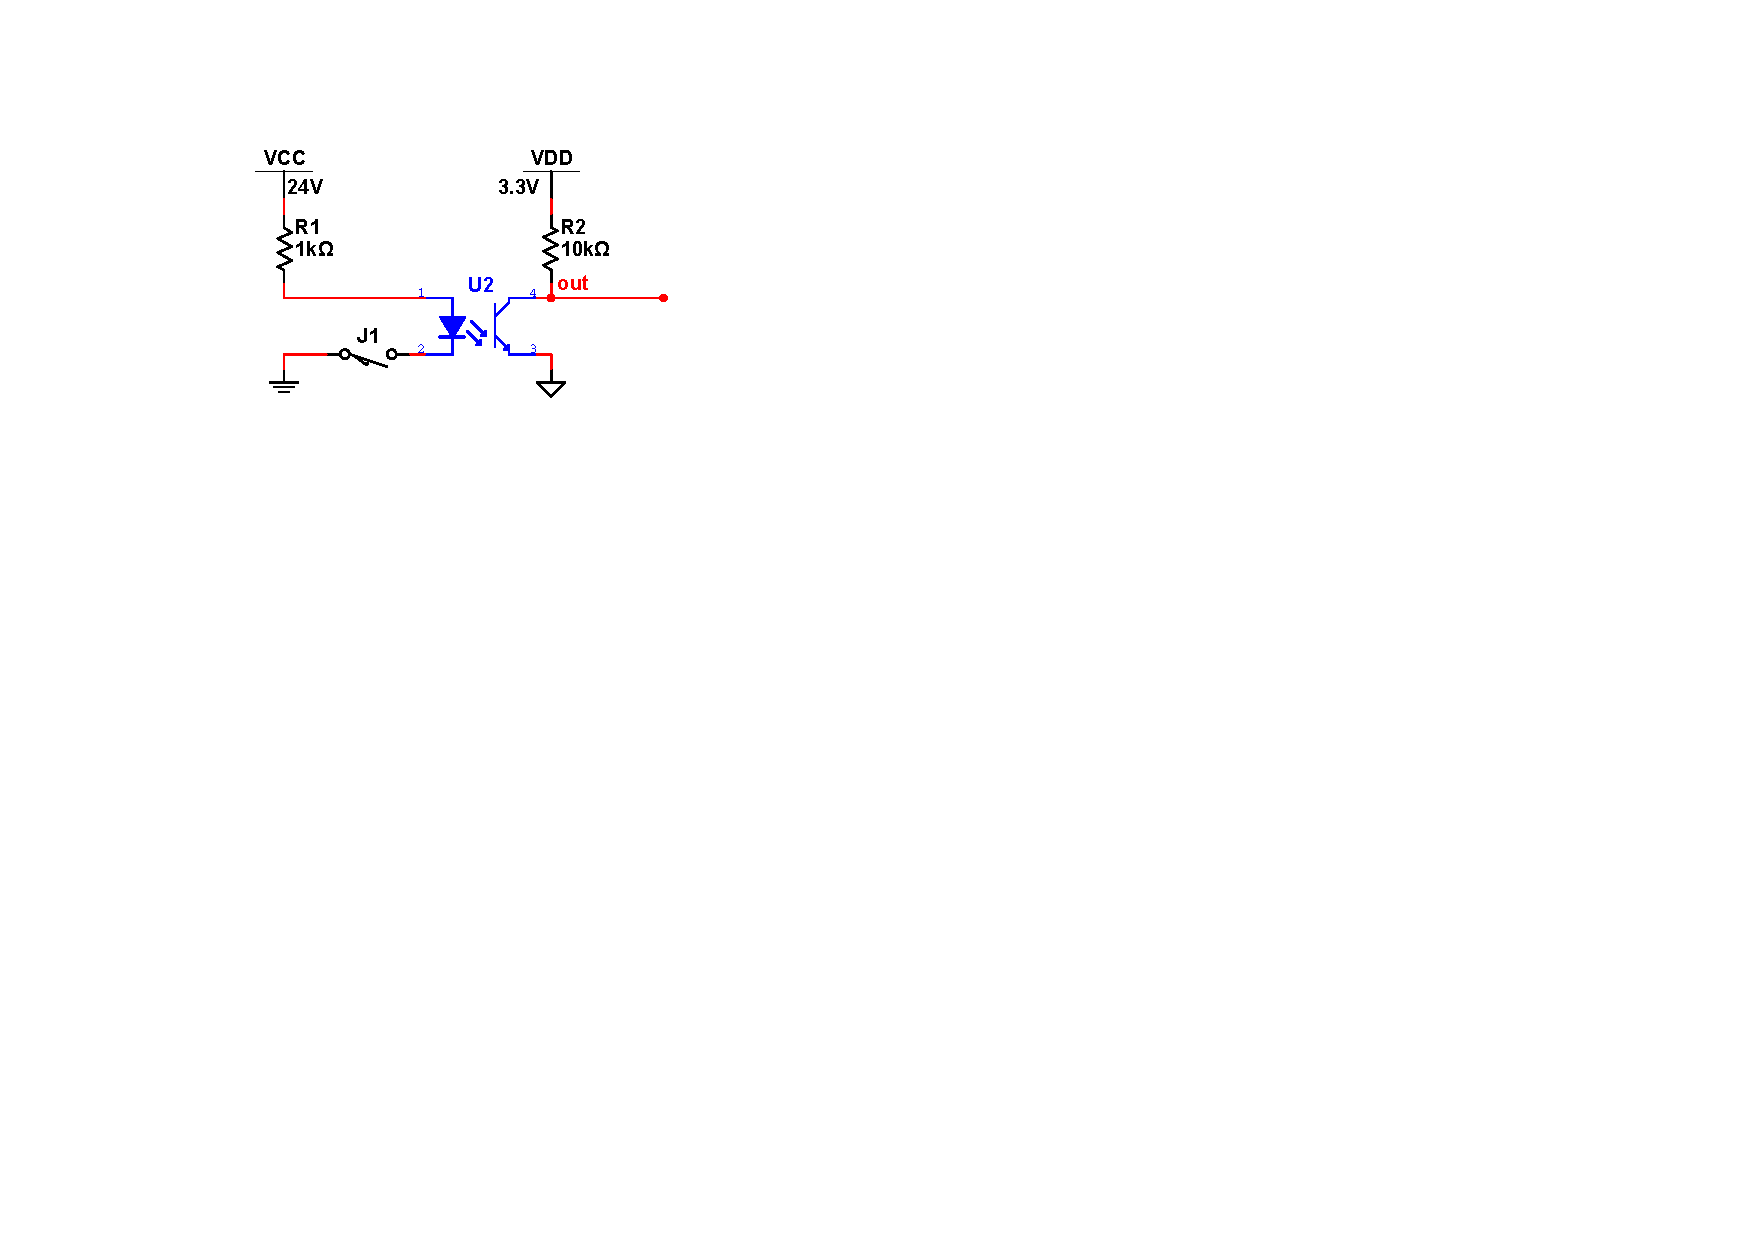
\includegraphics[width=0.5\linewidth]{rig/ctrl__intf__opto}
\caption{LAC-10A零位传感器接口原理图}
\label{fig:rig-ctrl-intf-opto}
\end{figure}

\subsection{微力传感器接口}\label{sec:rig-ctrl-intf-strain}

\ref{sec:rig-probe-sensor}节中选择的LSB200应变式微力传感器,其敏感元件为随受力变化而线性变化的电阻应变片,在内部接为电桥,如图~\ref{fig:rig-ctrl-strain-bridge}。电桥式传感器的基本原理如下:在\bverb|E+|、\bverb|E-|(E为excitation的缩写)两端加电压$V_{\mathrm{E}}$后,\bverb|S+|、\bverb|S-|(S为signal的缩写)两端电压为:
\[
V_{\mathrm{S}} = V_{\mathrm{E}} \cdot (\frac{R_2}{R_1 + R_2} - \frac{R_4}{R_3 + R_4})
\]
根据此关系,传感器被设计为满足:
\begin{equation}
\label{eq:rig-ctrl-intf-strain}
\frac{V_{\mathrm{S}}}{V_{\mathrm{E}}} = k (F + F_0)
\end{equation}
其中$F$为传感器受力,$k$为只与应变片本身特性相关的比例系数,$F_0$为传感器的零位偏差。

LSB200主要参数:阻值\SI{1000}{\ohm},标称满量程输出\SI{0.5}{\milli\volt\per\volt},最大激励电压\SI{10}{\volt}。由于电桥的等效输出电阻低,输出电压最大为\SI{5}{\milli\volt},需将该信号放大后处理。考虑到压强变送器内部采样率仅为\SI{50}{\hertz}(见\ref{sec:rig-ctrl-intf-loop}节),微力传感器无需高采样率;为简化电路,减小可能干扰脱附判断的噪声,选择专门为低速($\leq\SI{1}{\kilo\hertz}$)电桥设计的集成了可变增益仪表放大器与24位$\Sigma$--$\Delta$型ADC的AD7730芯片,如图~\ref{fig:rig-ctrl-ad7730-ac}。由于ADC的转换结果由其输入电压与参考电压的比值决定,一般必须使用精确电压基准芯片为ADC提供参考电压,才能得到准确的转换结果;但在本电路中,ADC参考电压与激励电压相同,均为$V_{\mathrm{E}}$,由\eqref{eq:rig-ctrl-intf-strain}式知,参考电压的变化不影响输入电压与参考电压的比值,即转换结果与参考电压具体取值无关,所以无需使用精确电压基准芯片。AD7730的参考电压名义值为\SI{5}{\volt},输入电压范围名义值(即放大器增益)可通过SPI接口设定为\SIlist[list-separator={、},list-final-separator={、或}]{\pm 10;\pm 20;\pm 40;\pm 80}{\milli\volt};当$V_{\mathrm{E}} = \SI{5}{\volt}$时,$V_{\mathrm{S}}$范围为\SI{\pm 2.5}{\milli\volt},因此设定AD7730的电压范围为\SI{\pm 10}{\milli\volt}。

\begin{figure}[p]
\centering
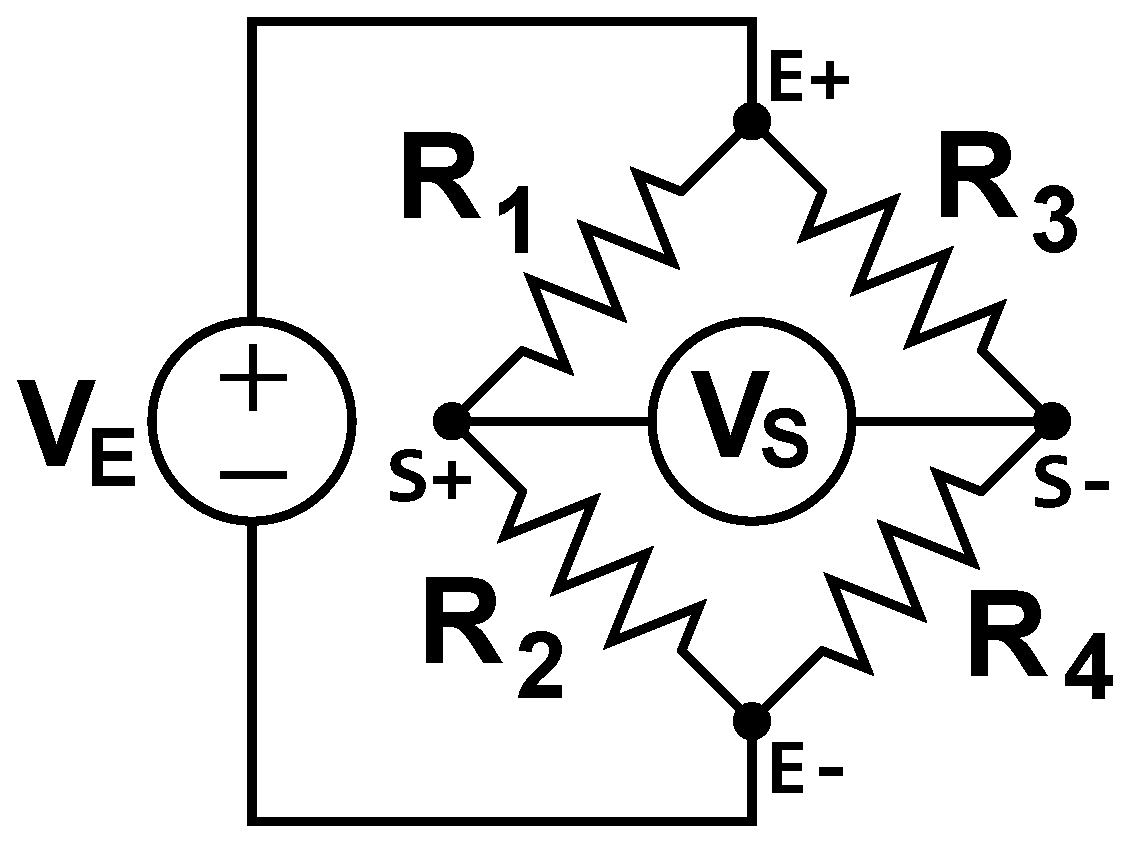
\includegraphics[width=0.4\linewidth]{rig/ctrl__intf__strain__bridge}
\caption{应变片电桥等效电路}
\label{fig:rig-ctrl-strain-bridge}
\end{figure}

\begin{sidewaysfigure}[p]
\centering
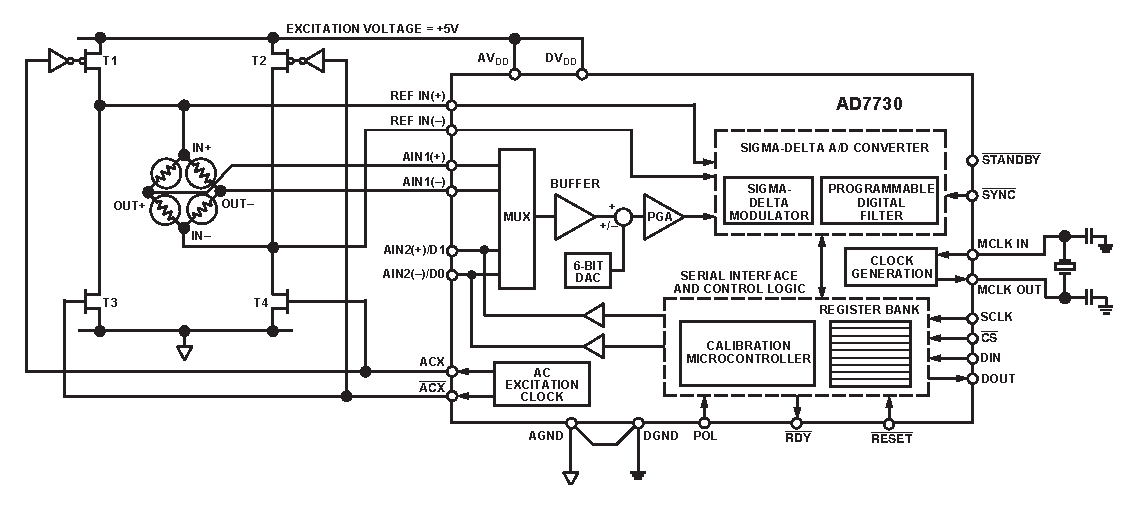
\includegraphics[width=1\linewidth]{rig/ctrl__intf__ad7730__ac}
\caption{AD7730电桥接口原理图}
\label{fig:rig-ctrl-ad7730-ac}
\end{sidewaysfigure}


\clearpage


\subsection{微控制器单元(MCU)}\label{sec:rig-ctrl-mcu}

由于电控系统无占用空间、耗电等特殊需求,选择常用的具有较强处理能力以及丰富外设的STM32F1系列ARM Cortex-M3内核32位MCU,以方便后续开发与扩展。结合图~\ref{fig:rig-ctrl-sch}以及各接口电路具体设计,规划MCU外设与针脚资源如图~\ref{fig:rig-ctrl-mcu-pinout}:\bverb|SPI1|及附近针脚连接压强采样ADC(AD7686,见\ref{sec:rig-ctrl-intf-loop}节),\bverb|SPI2|及附近针脚连接微力传感器采样ADC(AD7730,见\ref{sec:rig-ctrl-intf-strain}节);定时器\bverb|TIM4|向步进电机驱动器输出脉冲,外部中断\bverb|EXTI14|处理电动推杆零位传感器信号(\ref{sec:rig-ctrl-intf-stepper}节);\bverb|DAC|向电子比例阀接口(\ref{sec:rig-ctrl-intf-reg}节)提供设定点模拟信号;串口\bverb|USART1|与PC交换数据,\bverb|USART2|保留供MCU通过HART主机模块自动配置压强变送器,\bverb|USART3|保留供其他可能加入电控系统的串口外设使用。

\begin{figure}[tbhp]
\centering
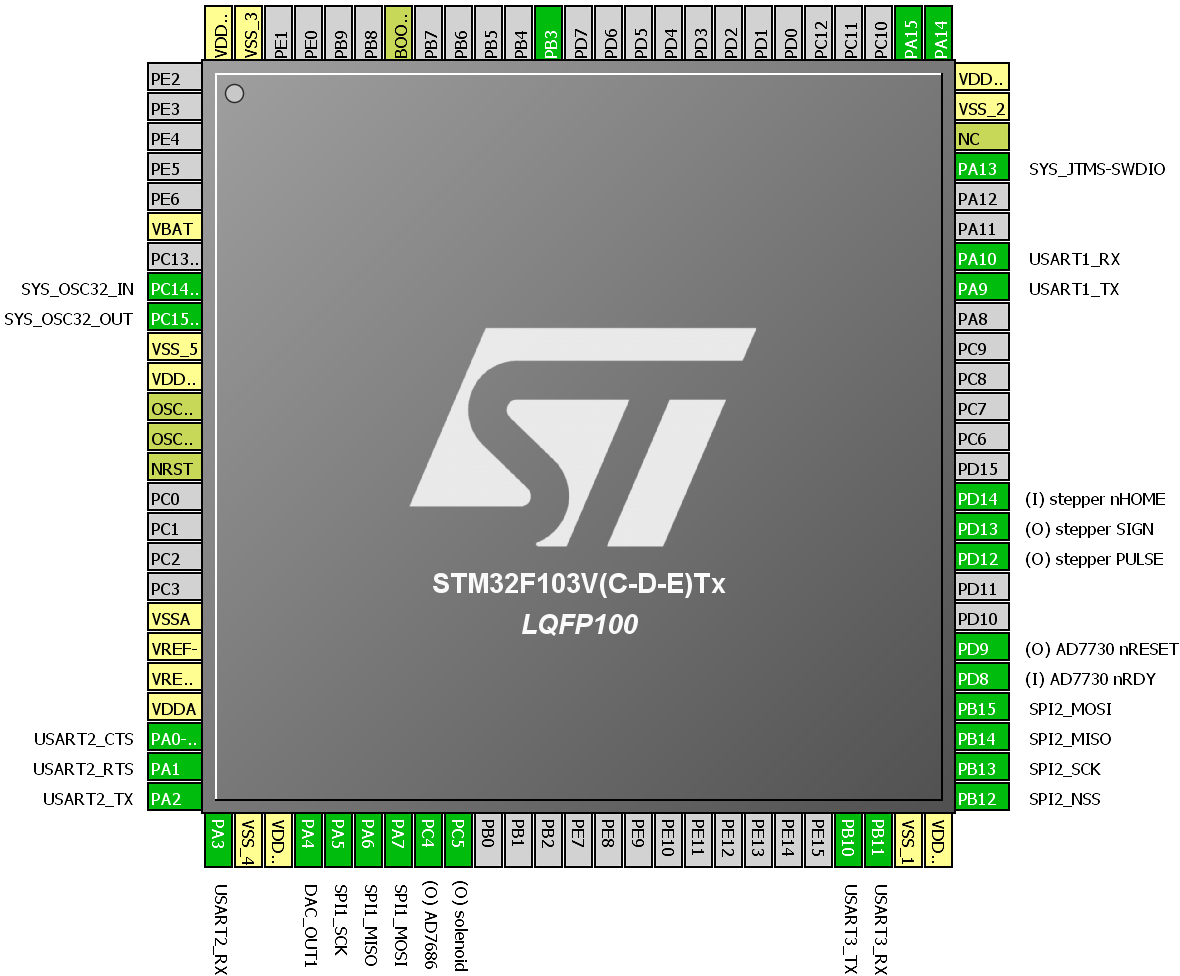
\includegraphics[width=1\linewidth]{rig/ctrl__mcu__pinout.png}
\caption{STM32F1外设与针脚资源分配图}
\label{fig:rig-ctrl-mcu-pinout}
\end{figure}

MCU的软件部分使用Keil RTX实时操作系统,系统定时器设为\SI{1}{\milli\second}周期,不同的控制过程在不同的操作系统线程(在RTX中称为``task'',即任务)中并发运行,互相可通过信号量(semaphore)、事件(event flag)等线程间通信手段实现信息传递与同步。其中:主线程负责与PC通信,接收PC传来的指令,协调其他线程,并将采集到的数据简单处理后传回PC;数据采集线程负责与AD7686与AD7730通信,协调同步采样时序;电动推杆控制线程负责向步进电机驱动器发送脉冲指令,记录电动推杆位置,实现自动回零等;DAC控制线程负责向电子比例阀输出平缓上升的斜坡信号。以下重点讨论较为复杂的数据采集与电动推杆控制部分。

\subsubsection{数据采集部分}\label{sec:rig-ctrl-mcu-adc}

首先确定采样率。AD768x系列允许的最大采样率至少为\SI{100}{\kilo\hertz},而压强变送器本身的输出更新速率为\SI{50}{\hertz},因此可以适当过采样以提高ADC有效精度。AD7730的采样率可通过SPI接口配置,最高可达\SI{1}{\kilo\hertz},且由于AD7730为$\Sigma$--$\Delta$型ADC,其采样率越低,有效精度越高。为简化实现,将两ADC的采样率均定为\SI{100}{\hertz},这样即可实现同步采样:AD7686的采样由其\bverb|CNV|引脚上升沿控制,即采样率由外部决定,而AD7730的采样率由其内部时钟与配置寄存器决定;因此可使用AD7730的中断请求引脚\bverb|nRDY|作为同步信号,触发转换与读取时序如图~\ref{fig:rig-ctrl-mcu-adc-timing}:中断响应后,立刻开始AD7686转换,并同时开始读取AD7730数据;当AD7730数据读取完毕时,AD7686转换已完成,可继续读取AD7686数据。

\begin{figure}[tbh]
\centering
\begin{minipage}{1\textwidth}
\resizebox{1\textwidth}{!}{
\begin{tikztimingtable}
  [ timing/font=\ttfamily
  , timing/slope=0.2
  , timing/coldist=12pt % column distance
  , timing/c/arrow pos=0.7
  , timing/c/arrow tip=stealth
  , xscale=0.6, yscale=1.5
  , thick
  ]
{AD7730 nRDY}  & []
  H 2L L;
  7{2L} 8{2E} 1{2H};
  H;
  32H;
  H ; [dotted] 3H; \\
{AD7730 nCS\ } & []
  H 2H L;
  32L;
  H;
  32H;
  H; [dotted]3H; \\
{AD7730 SCLK}  & [timing/c/falling arrows]
  L 2L L;
  32{C};
  L;
  32L;
  L; [dotted] 3L; \\
{AD7730 MISO}  & []
  Z 2Z Z;
  32b{1}{16-bit\footnotemark[1]{} data}{1};
  Z;
  32Z;
  Z; [dotted] 3Z; \\
\\
{AD7686 CNV\ } & []
  L 2L H;
  32H;
  L;
  32L;
  L; [dotted] 3L; \\
{AD7686 SCK\ } & [timing/c/rising arrows]
  L 2L L;
  32L;
  L;
  0C0C 32{C};
  L; [dotted] 3L; \\
{AD7686 MISO}  & []
  Z 2Z Z;
  32Z;
  0.5Z;
  32b{1}{16-bit data}{1};
  1.5Z; [dotted] 3Z; \\
\extracode
  \begin{scope}[on background layer, help lines]
    \vertlines[red, semithick]{1.1}
    \vertlines[olive, semithick]{3.2,36.0}
  \end{scope}
\end{tikztimingtable}
}

\footnotetext[1]{受各种噪声影响,实际有效位数略低于16位,因此将AD7730配置为16位输出。}

\end{minipage}
\caption{ADC通信时序}
\label{fig:rig-ctrl-mcu-adc-timing}
\end{figure}

\subsubsection{电动推杆控制部分}\label{sec:rig-ctrl-mcu-stepper}

由\ref{sec:rig-probe-feeding}节讨论知,电动推杆的主要作用为控制微力探头与晶圆接触。在此之前,需先将电动推杆移动到其零位,即推杆最短的位置。由于零位传感器存在一定滞回(见\ref{sec:rig-ctrl-intf-stepper}节),采用如下步骤回零:首先,若零位传感器处于未动作状态,则快速驱动电动推杆缩短,直至零位传感器动作;然后,以稍慢的速度驱动电动推杆伸长,直至零位传感器不再动作;最后,缓慢驱动电动推杆缩短,直至零位传感器再次动作;此时可认为电动推杆处于确定的零位。与电机驱动器的底层接口方面,由于电动推杆只需缓慢匀速运动,直接使用MCU内置定时器输出固定频率的脉冲即可实现。另外,为防止意外造成电动推杆超过其行程,在回零之后,需持续记录已发送的脉冲数,在预计推杆即将超过行程时停止运动。


\section{本章小结}\label{sec:rig-summary}

%TODO:summary